\documentclass{beamer}

\usepackage[utf8]{inputenc}
\usepackage[T1]{fontenc}
\usepackage[french]{babel}
\usepackage[babel=true]{csquotes} % guillements français
\usepackage{graphicx}
\graphicspath{{Images/}{Images/L3_Android/}}
\usepackage{color}
\usepackage{hyperref}
\hypersetup{colorlinks,linkcolor=,urlcolor=blue}


\mode<presentation>
{
  %% PLUSIEURS THEMES EXISTENT : VOIR DOCUMENTATION
  % \usetheme{Warsaw}
  % \usetheme{Frankfurt}
  \usetheme{Madrid}
  % or ...

  \setbeamercovered{transparent}
  % or whatever (possibly just delete it)
}


\title[Dev. Mobiles -- L3 info]{Développement pour mobiles\\L3 Informatique\\\textbf{Jeu de dame}}
\author{Billy Ronico, Ismael Saïd}
\institute[DI]{Université de la Réunin}
\date{\today}


\subject{Talks}
% This is only inserted into the PDF information catalog. Can be left
% out.



% If you have a file called "university-logo-filename.xxx", where xxx
% is a graphic format that can be processed by latex or pdflatex,
% resp., then you can add a logo as follows:

% \pgfdeclareimage[height=0.5cm]{university-logo}{university-logo-filename}
% \logo{\pgfuseimage{university-logo}}



% Delete this, if you do not want the table of contents to pop up at
% the beginning of each subsection:
\AtBeginSection[]
{
  \begin{frame}<beamer>
    \frametitle{Plan}
    \tableofcontents[currentsection]
  \end{frame}
}

% \AtBeginSubsection[]
% {
%   \begin{frame}<beamer>
%     \frametitle{Plan}
%     \tableofcontents[currentsection,currentsubsection]
%   \end{frame}
% }


% If you wish to uncover everything in a step-wise fashion, uncomment
% the following command:

%\beamerdefaultoverlayspecification{<+->}


\begin{document}

\begin{frame}
  \titlepage
\end{frame}


%%%%%%%%%%%%%%%%%%%%
\section{Introduction}
%%%%%%%%%%%%%%%%%%%%
%
%
\begin{frame}
  \frametitle{Presentation du jeu}
    \subsection{Presentation du jeu}
    Le jeu de dame est un jeu de strategie qui date du debut du 18 ème siècle. 
    
    Il se joue sur un damier de taille n * n (en général 10 * 10).

    L'objéctif du jeu est de prendre tout les pions adverses.

\end{frame}
%
%
\begin{frame}
  \frametitle{Presentation du jeu}

  \begin{center}
    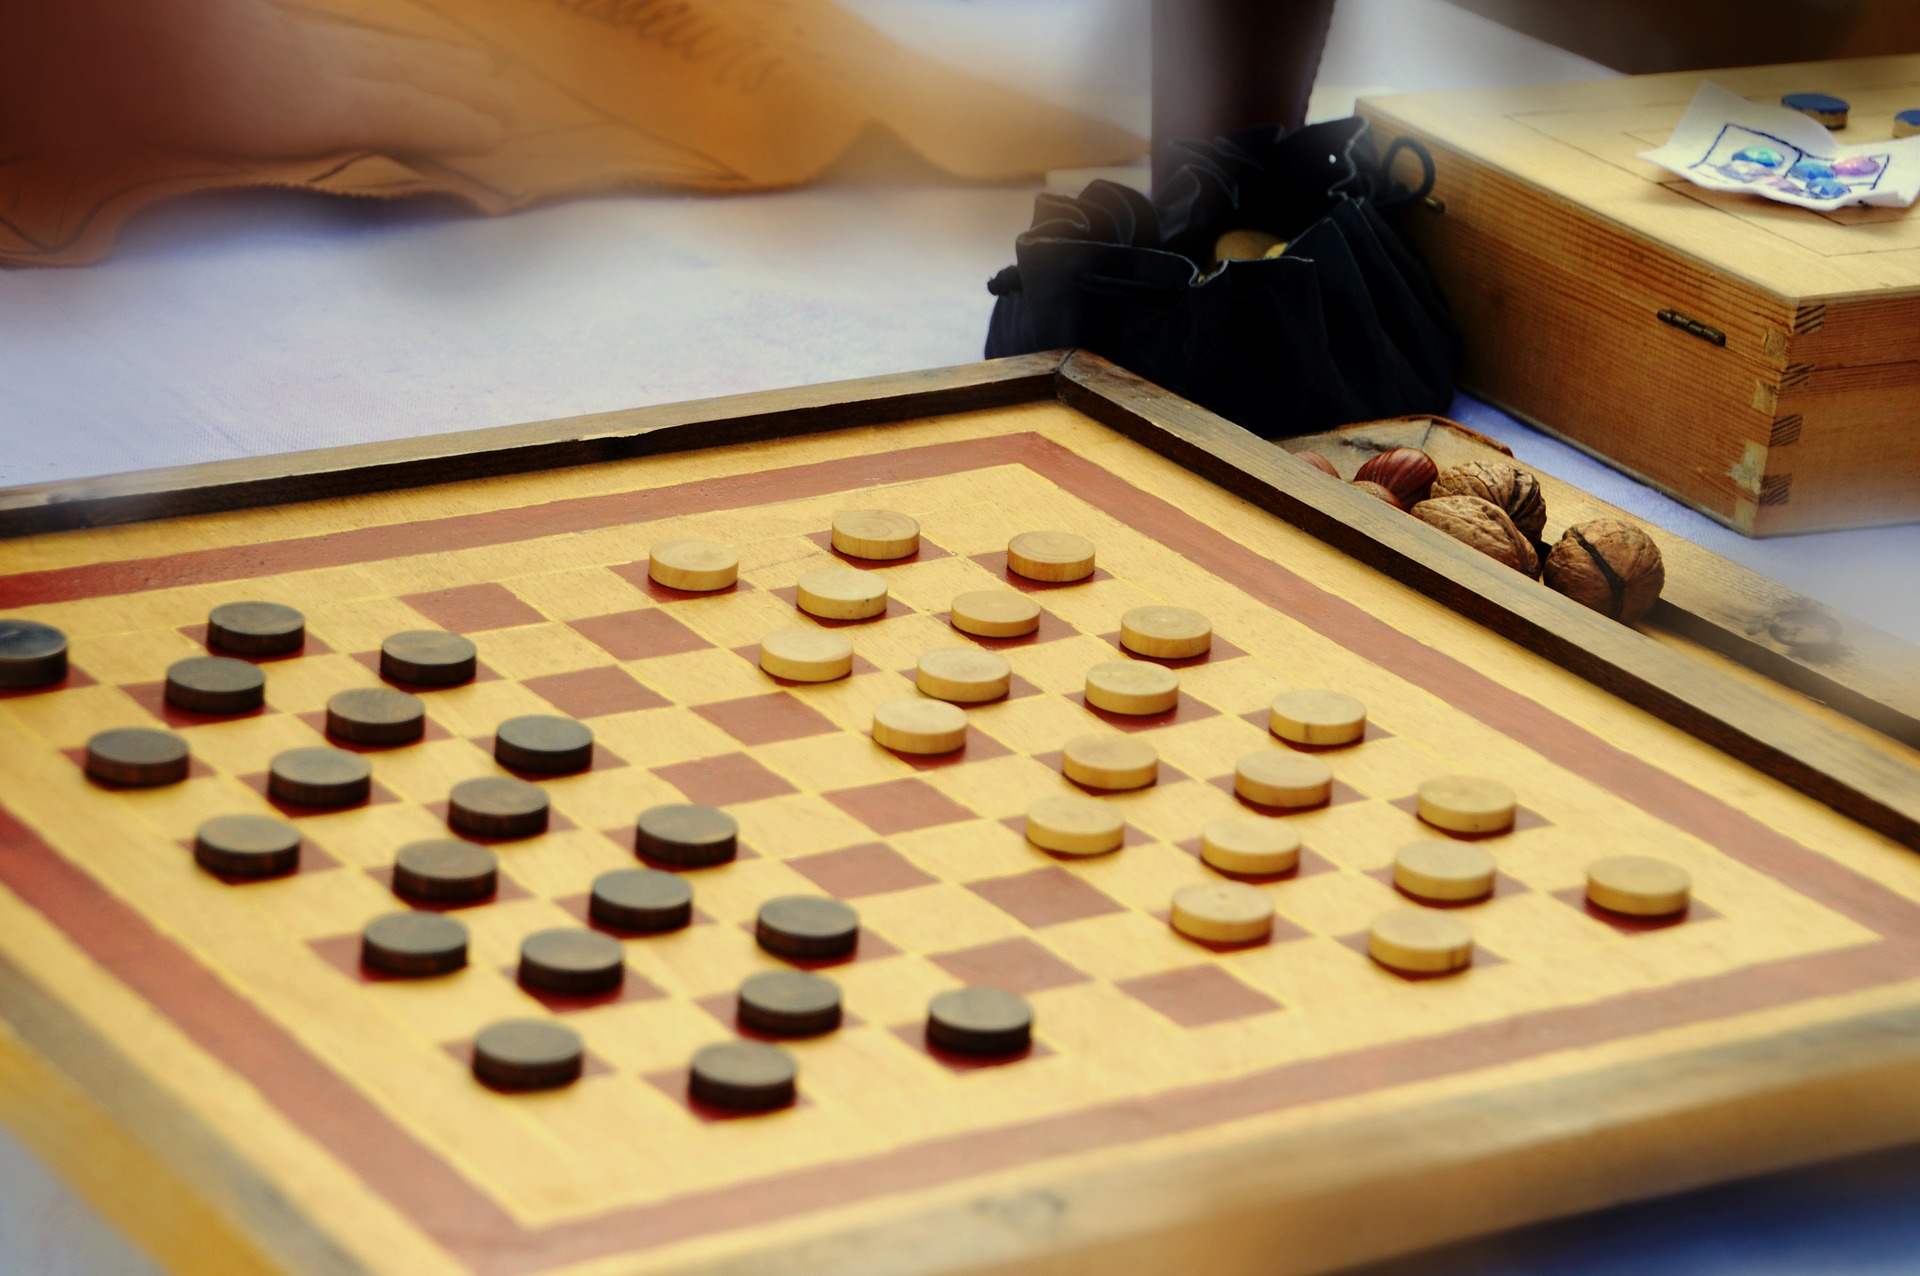
\includegraphics[scale=0.5]{img_dame.jpg}
  \end{center}
  
  \begin{center}
    Jeu de dame
  \end{center}

\end{frame}

\begin{frame}

  \frametitle{Règles de jeu}

  \subsection{Règles de jeu}

  \begin{itemize}
    \item Le jeu se joue à 2 joueurs sur un plateau de taille n * n.
    \item Les joueurs jouent chacun à leur tour. Les blancs commencent toujours.
    \item Le but du jeu est de capturer tous les pions adverses. 
    \item Si un joueur ne peut plus bouger, même s'il lui reste des pions, il perd la partie. 
    \item Chaque pion peut se déplacer d'une case vers l'avant en diagonale. 
    \item Un pion arrivant sur la dernière rangée et s'y arrêtant est promu en « dame ».
    \item La dame se déplace sur une même diagonale d'autant de cases qu'elle le désire, en avant et en arrière.
  
  \end{itemize}

\end{frame}

\begin{frame}
  \frametitle{Règles de jeu}
  \begin{itemize}
    \item Un pion peut en prendre un autre en sautant par dessus le pion adverse
     pour se rendre sur la case vide située derrière celui-ci. Le pion sauté est retiré du jeu.
    \item La prise est obligatoire.
    \item Lorsque plusieurs prises sont possibles, 
    il faut toujours prendre du côté du plus grand nombre de pièces.
    \item La dame doit prendre tout pion situé sur sa diagonale 
    (s'il y a une case libre derrière) et doit changer de direction à chaque 
    fois qu'une  nouvelle prise est possible. 
  \end{itemize}
\end{frame}

\section{Presentation de l'application}

\begin{frame}
  \frametitle{Menu principal - smartphone}
  \subsection{Menu principal}

  \begin{center}
    Jeu old school <==> Design old school
  \end{center}

  \begin{center}
    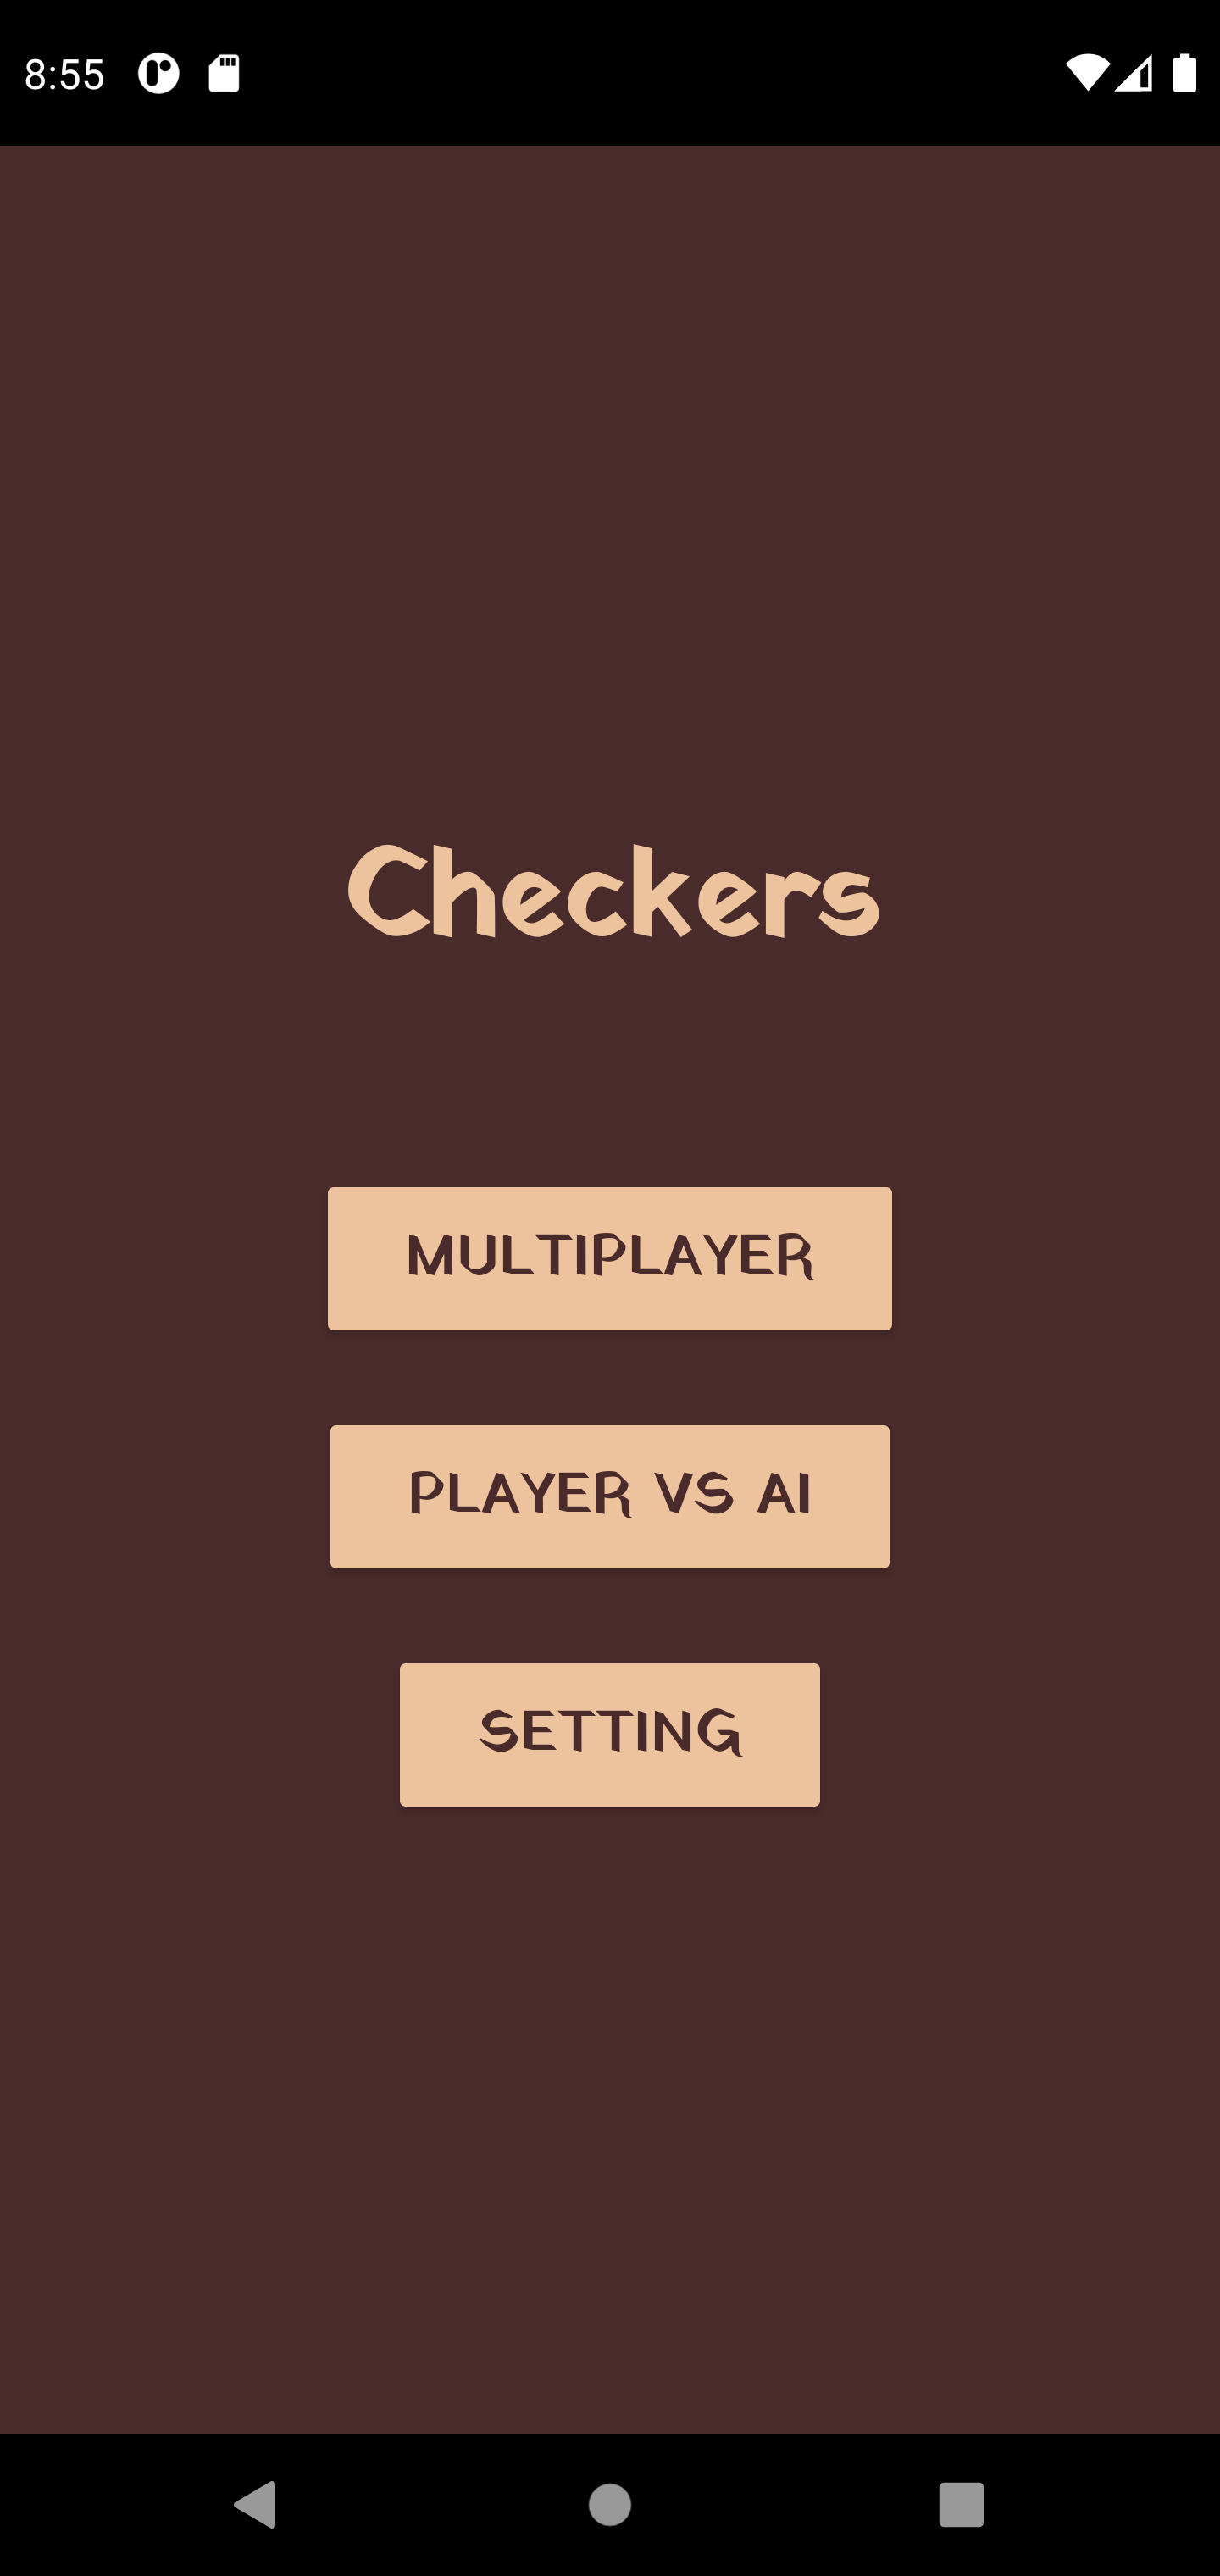
\includegraphics[scale=0.05]{menu_principal.png}
    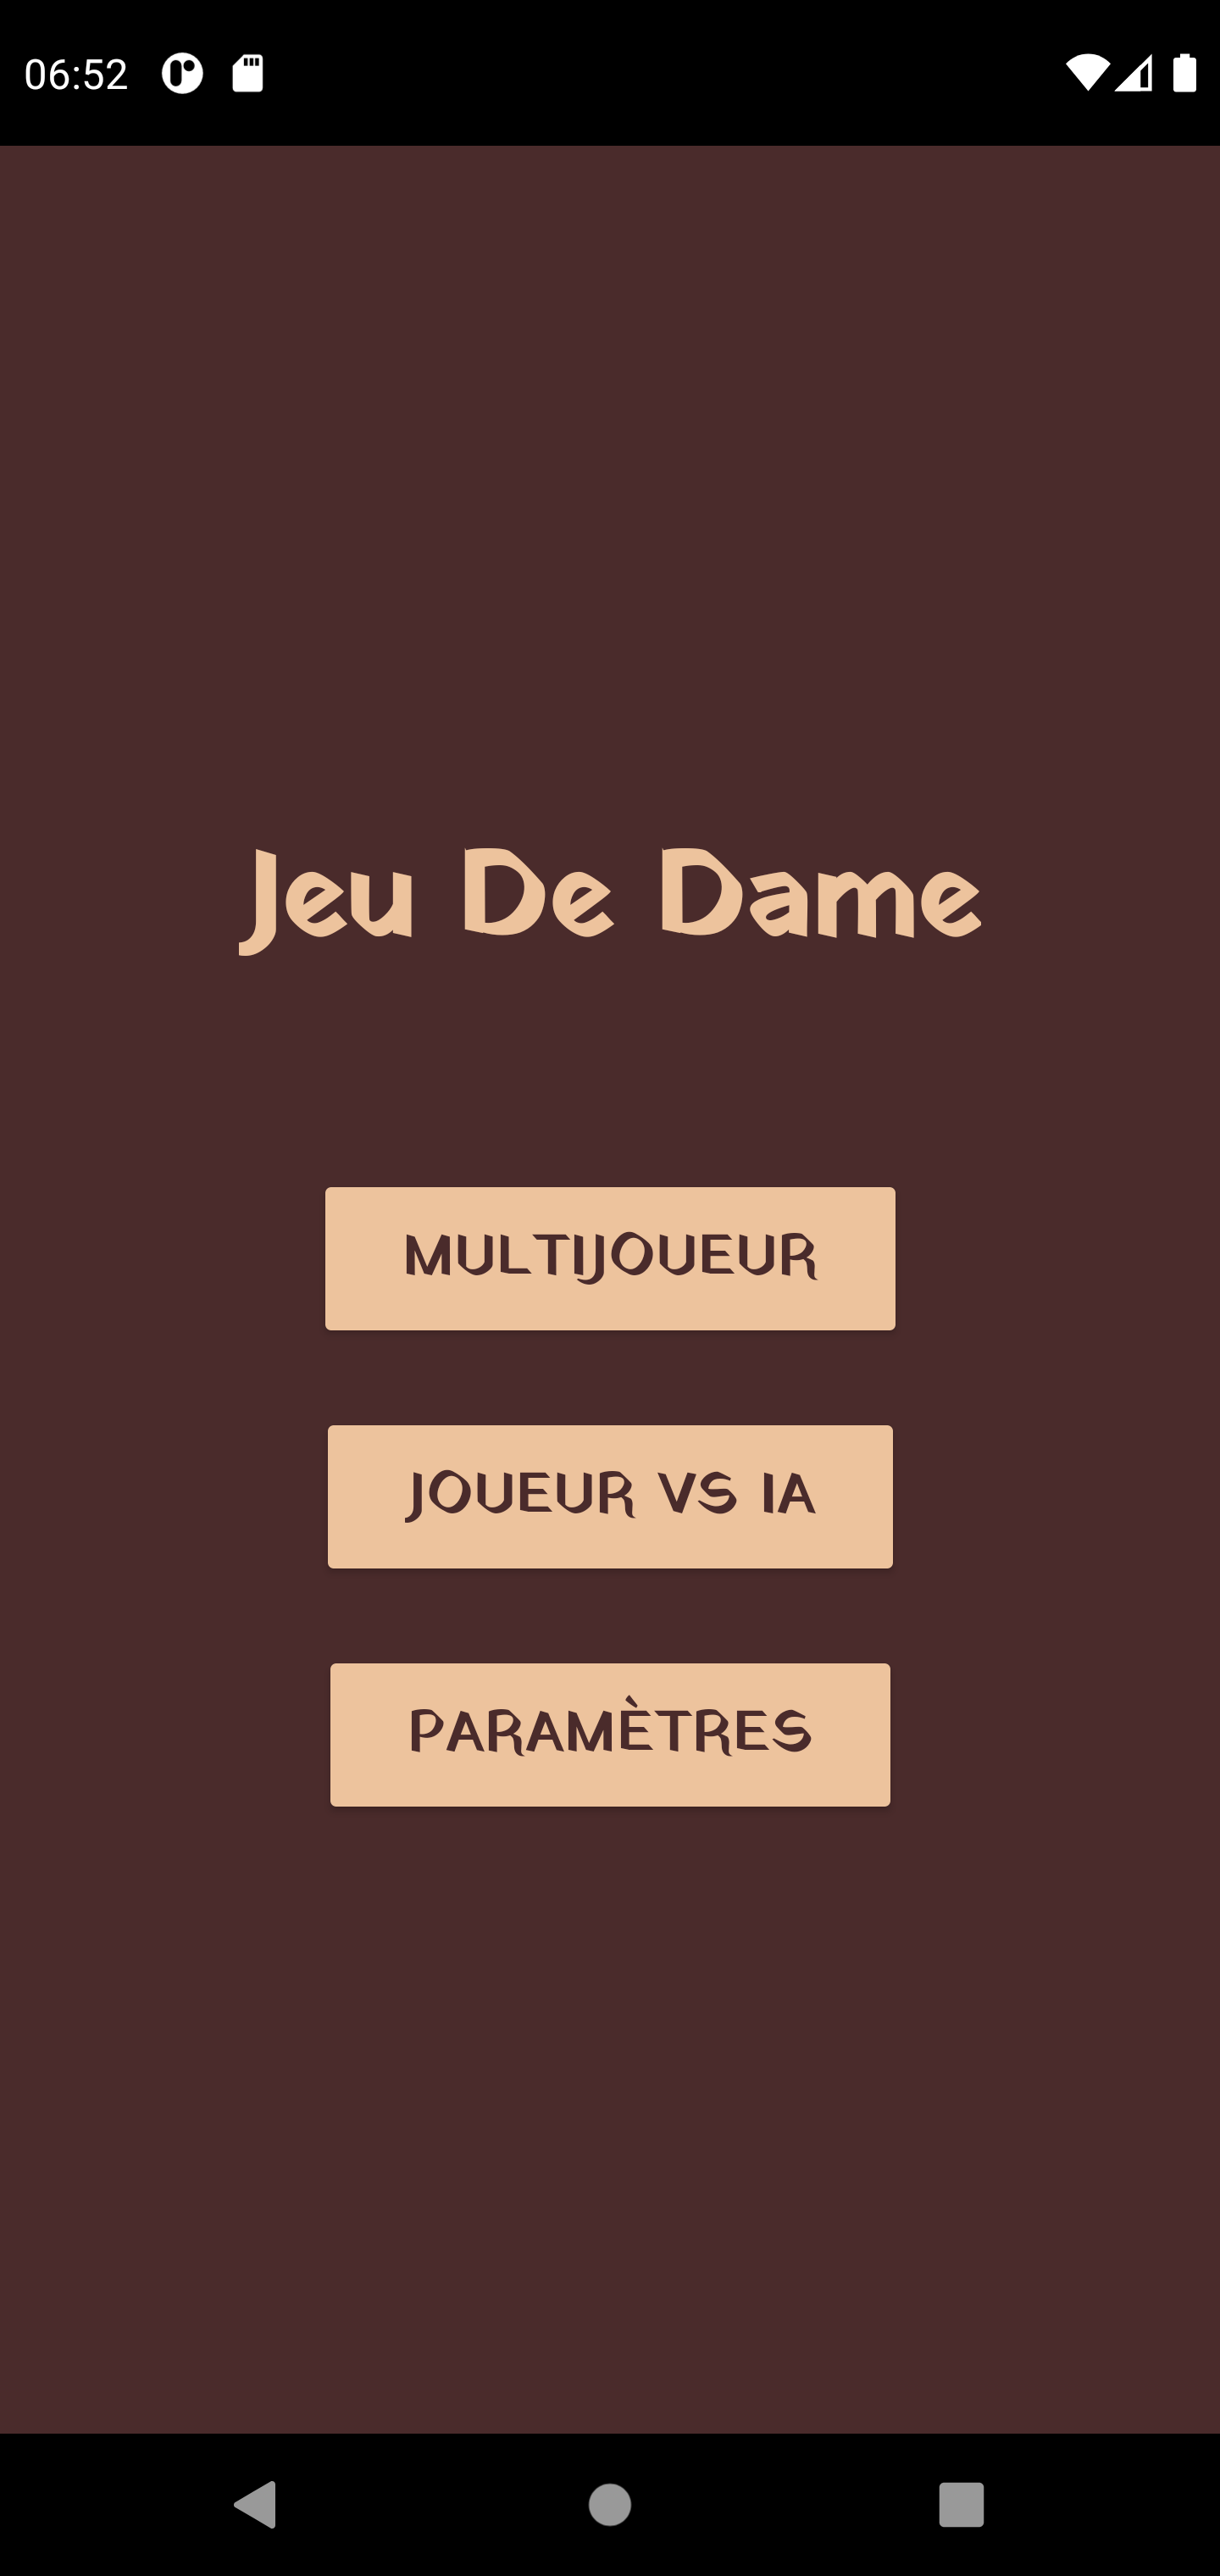
\includegraphics[scale=0.05]{menu_fr.png}
  \end{center}

  Le menu principal est disponible en \textbf{"Français"} et en \textbf{"Anglais"}

\end{frame}

\begin{frame}
  \frametitle{Menu principal - tablette}

  \begin{center}
    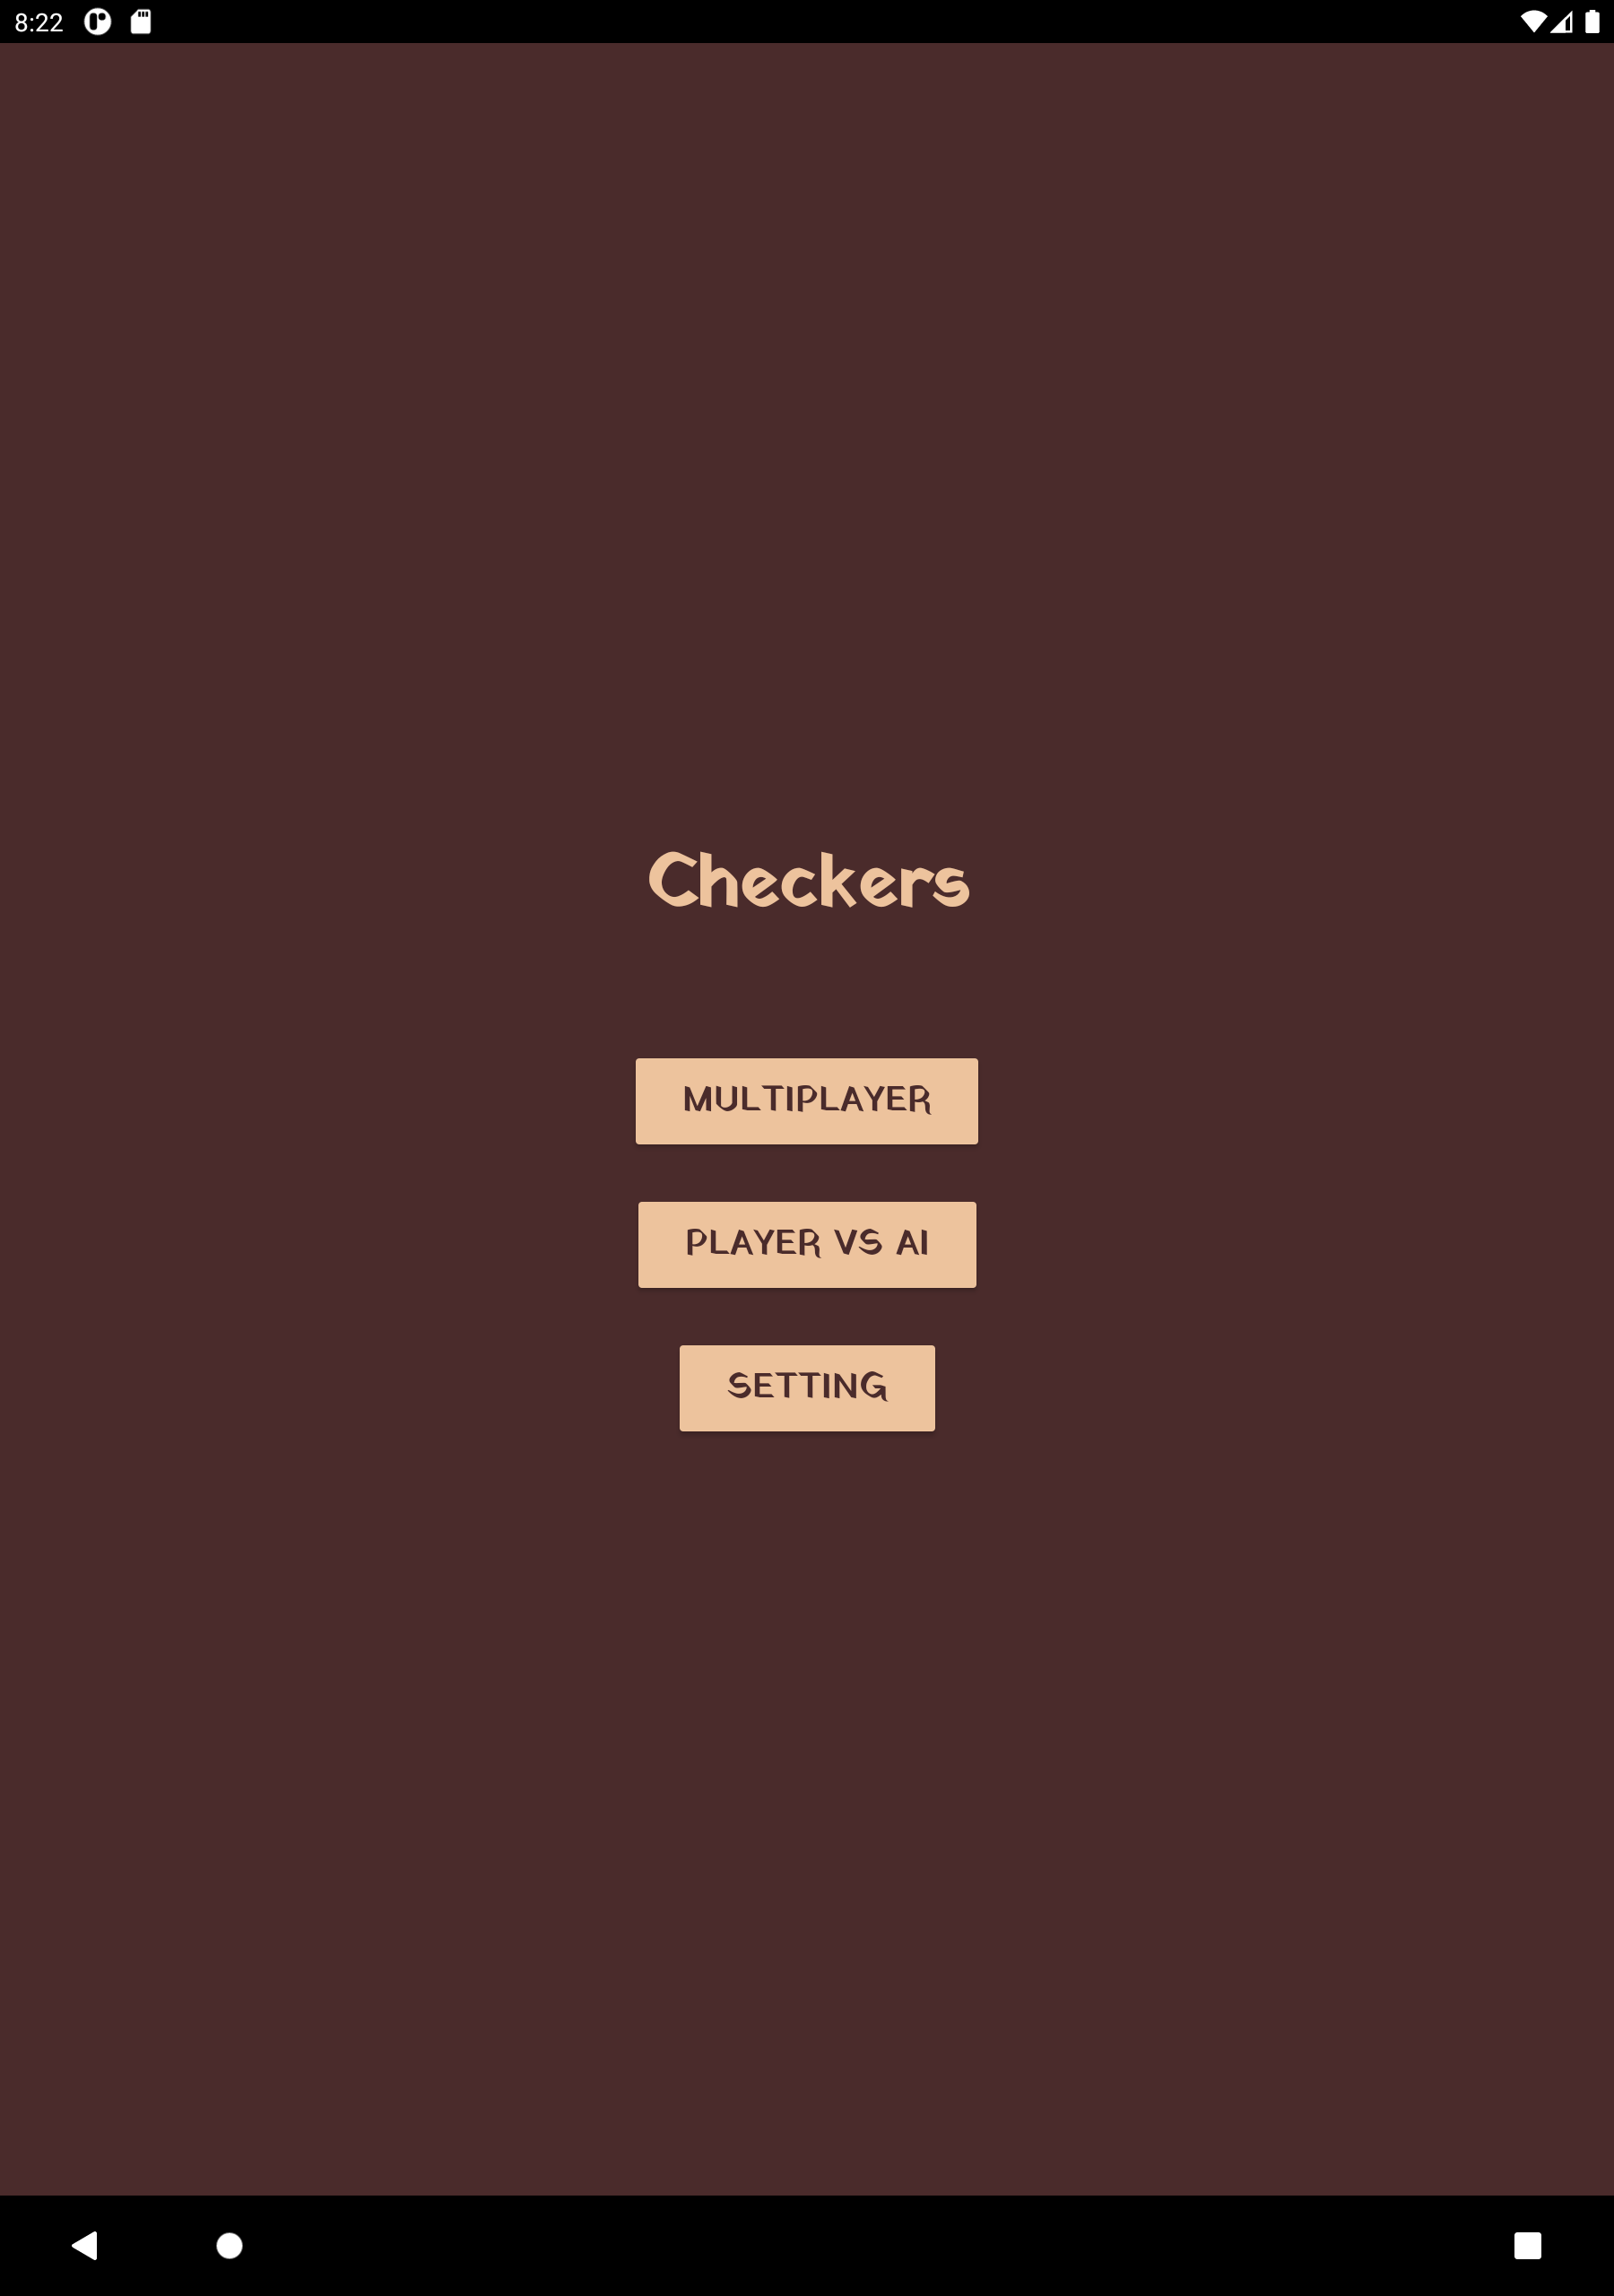
\includegraphics[scale=0.06]{menu_tablet.png}
  \end{center}

  \begin{center}
    Le menu est totalement \textbf{responsive}
  
    Utilisation de \textbf{ConstraintLayout}
  \end{center}

\end{frame}

\begin{frame}
  \frametitle{Paramètre - smartphone}
  \subsection{Paramètre}
  \begin{center}
    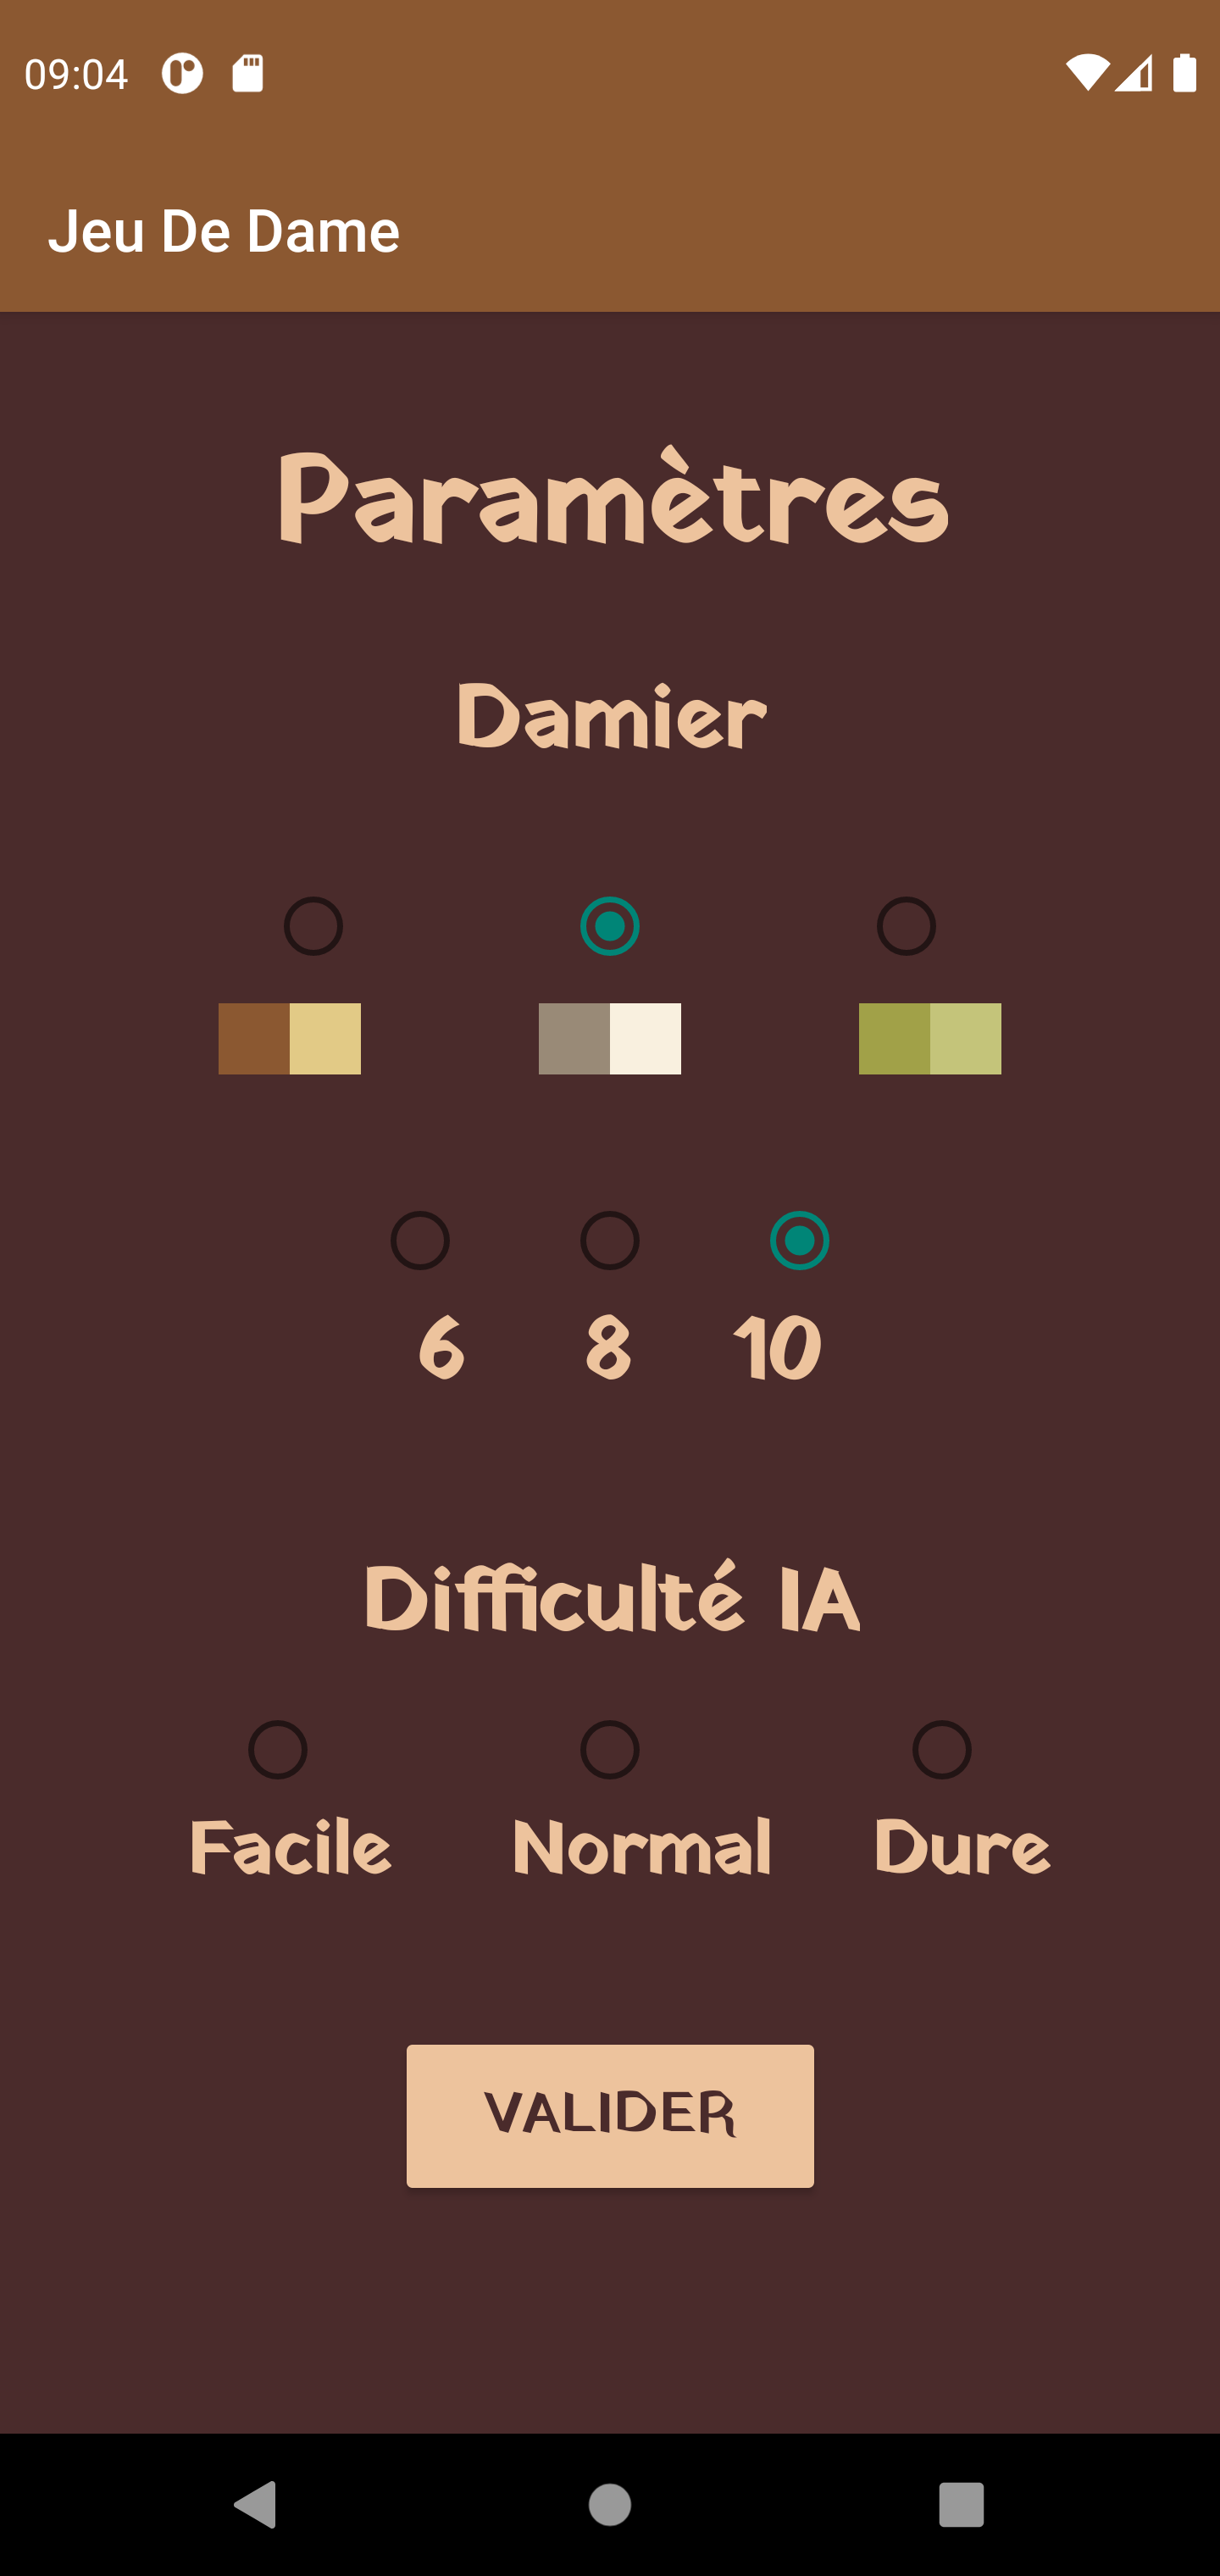
\includegraphics[scale=0.05]{setting_francais.png}
    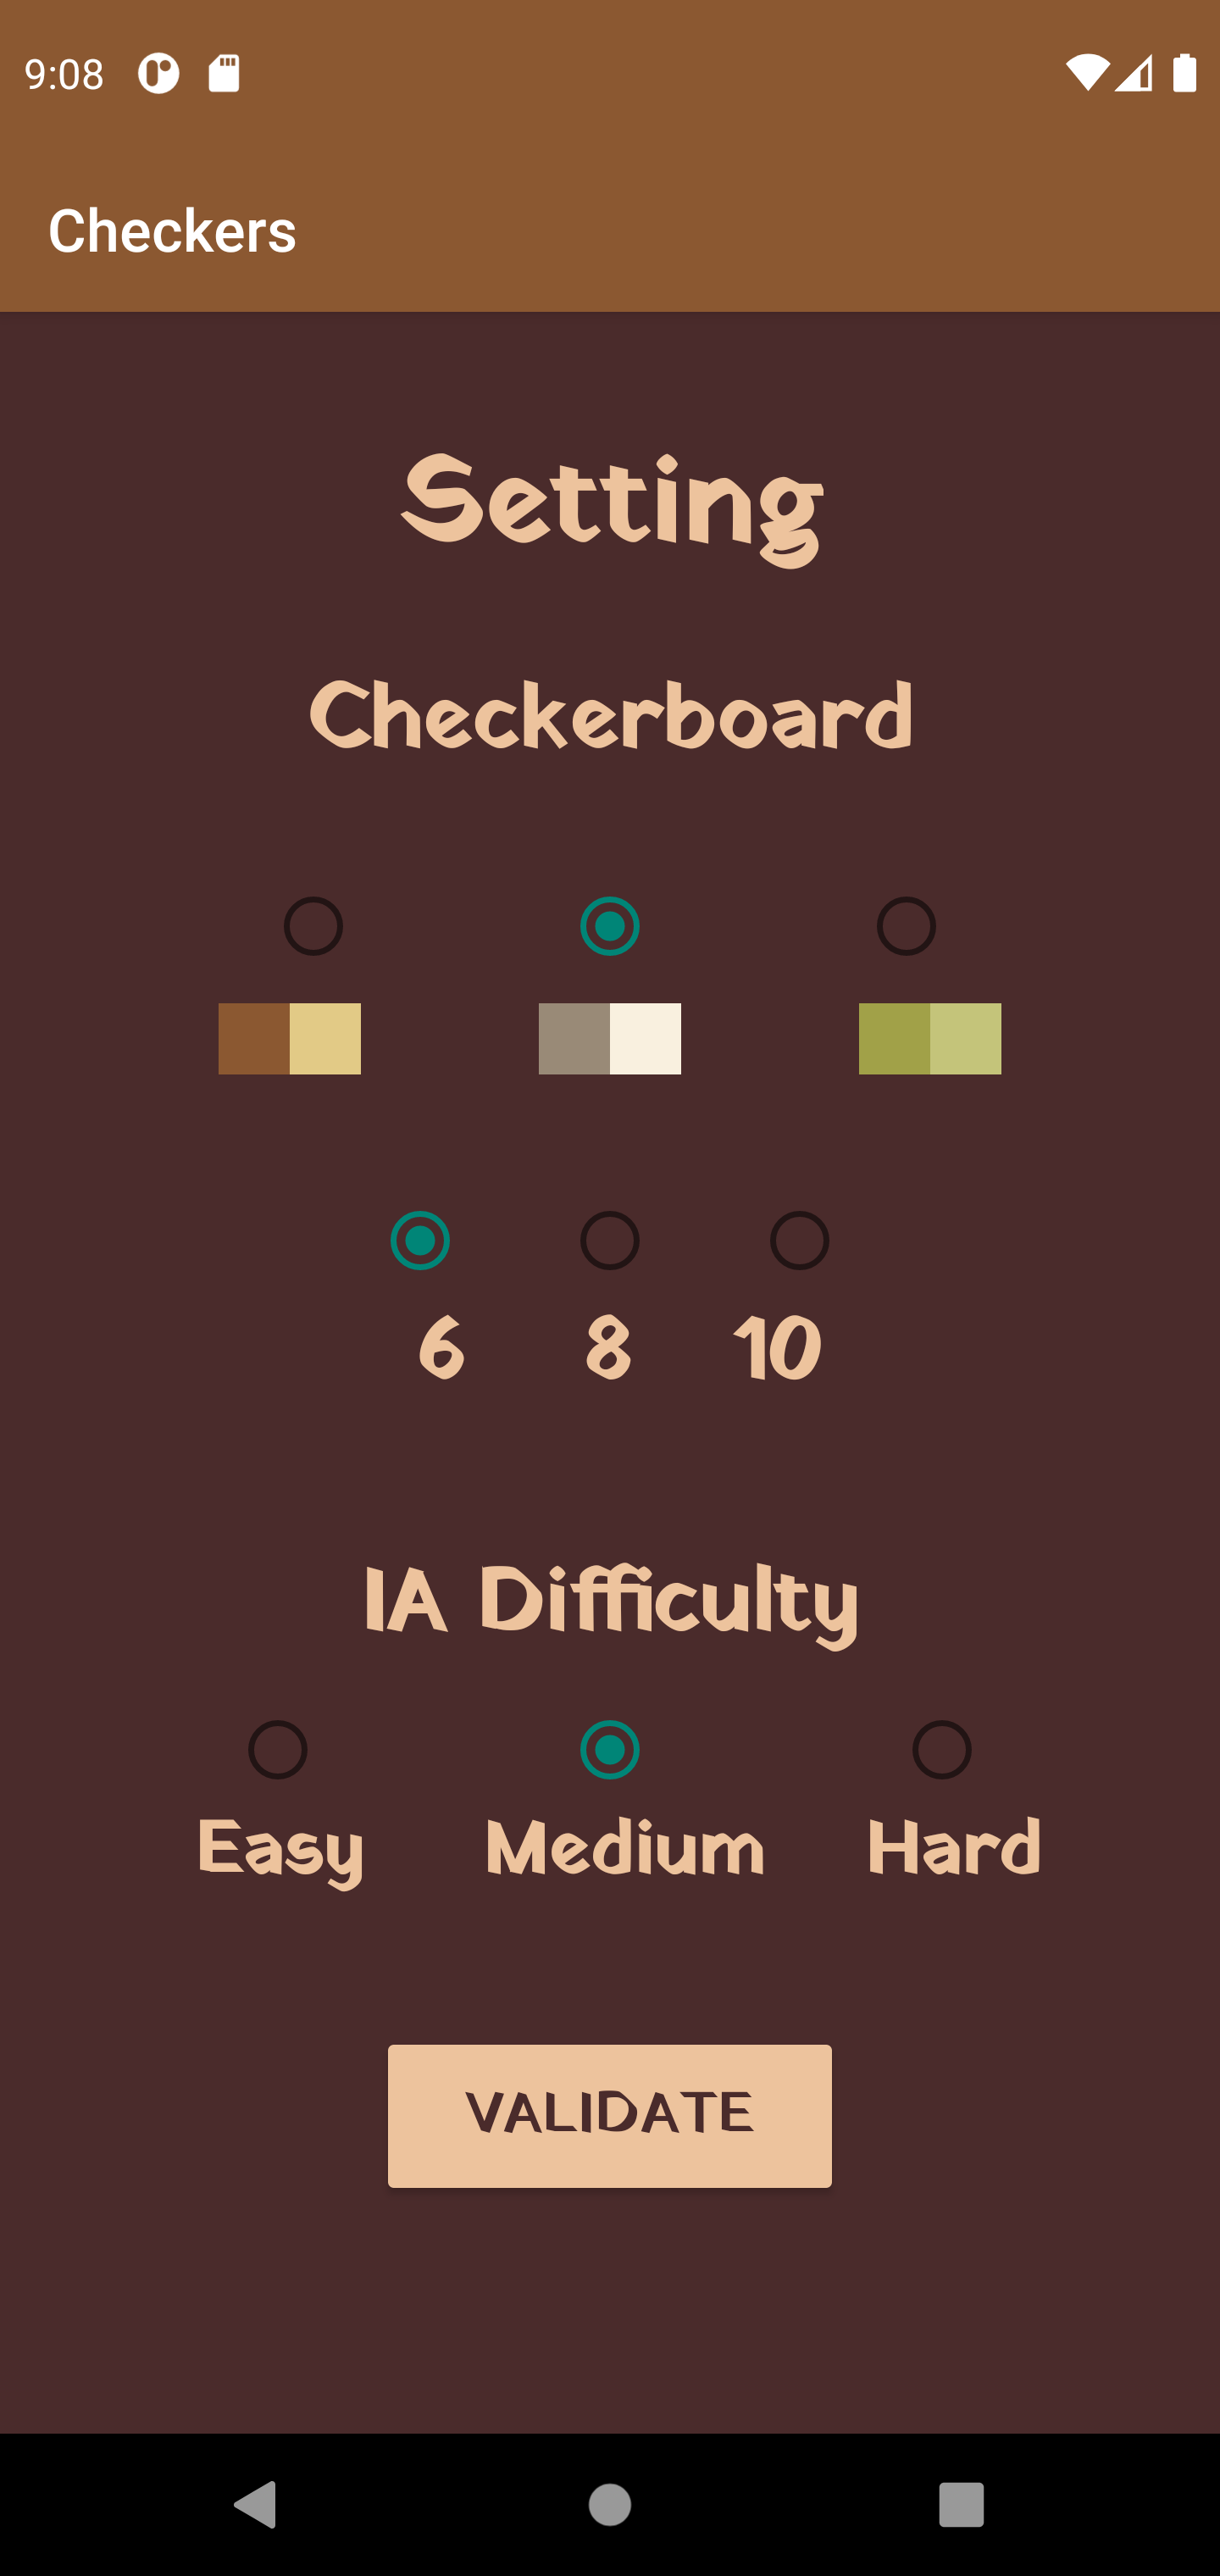
\includegraphics[scale=0.05]{setting_en.png}
  \end{center}

  \begin{center}
    Les paramètres seront ensuite stoqués 
    dans un fichier pour la persistance des données
  \end{center}

\end{frame}

\begin{frame}
  \frametitle{Paramètre - tablette}

  \begin{center}
    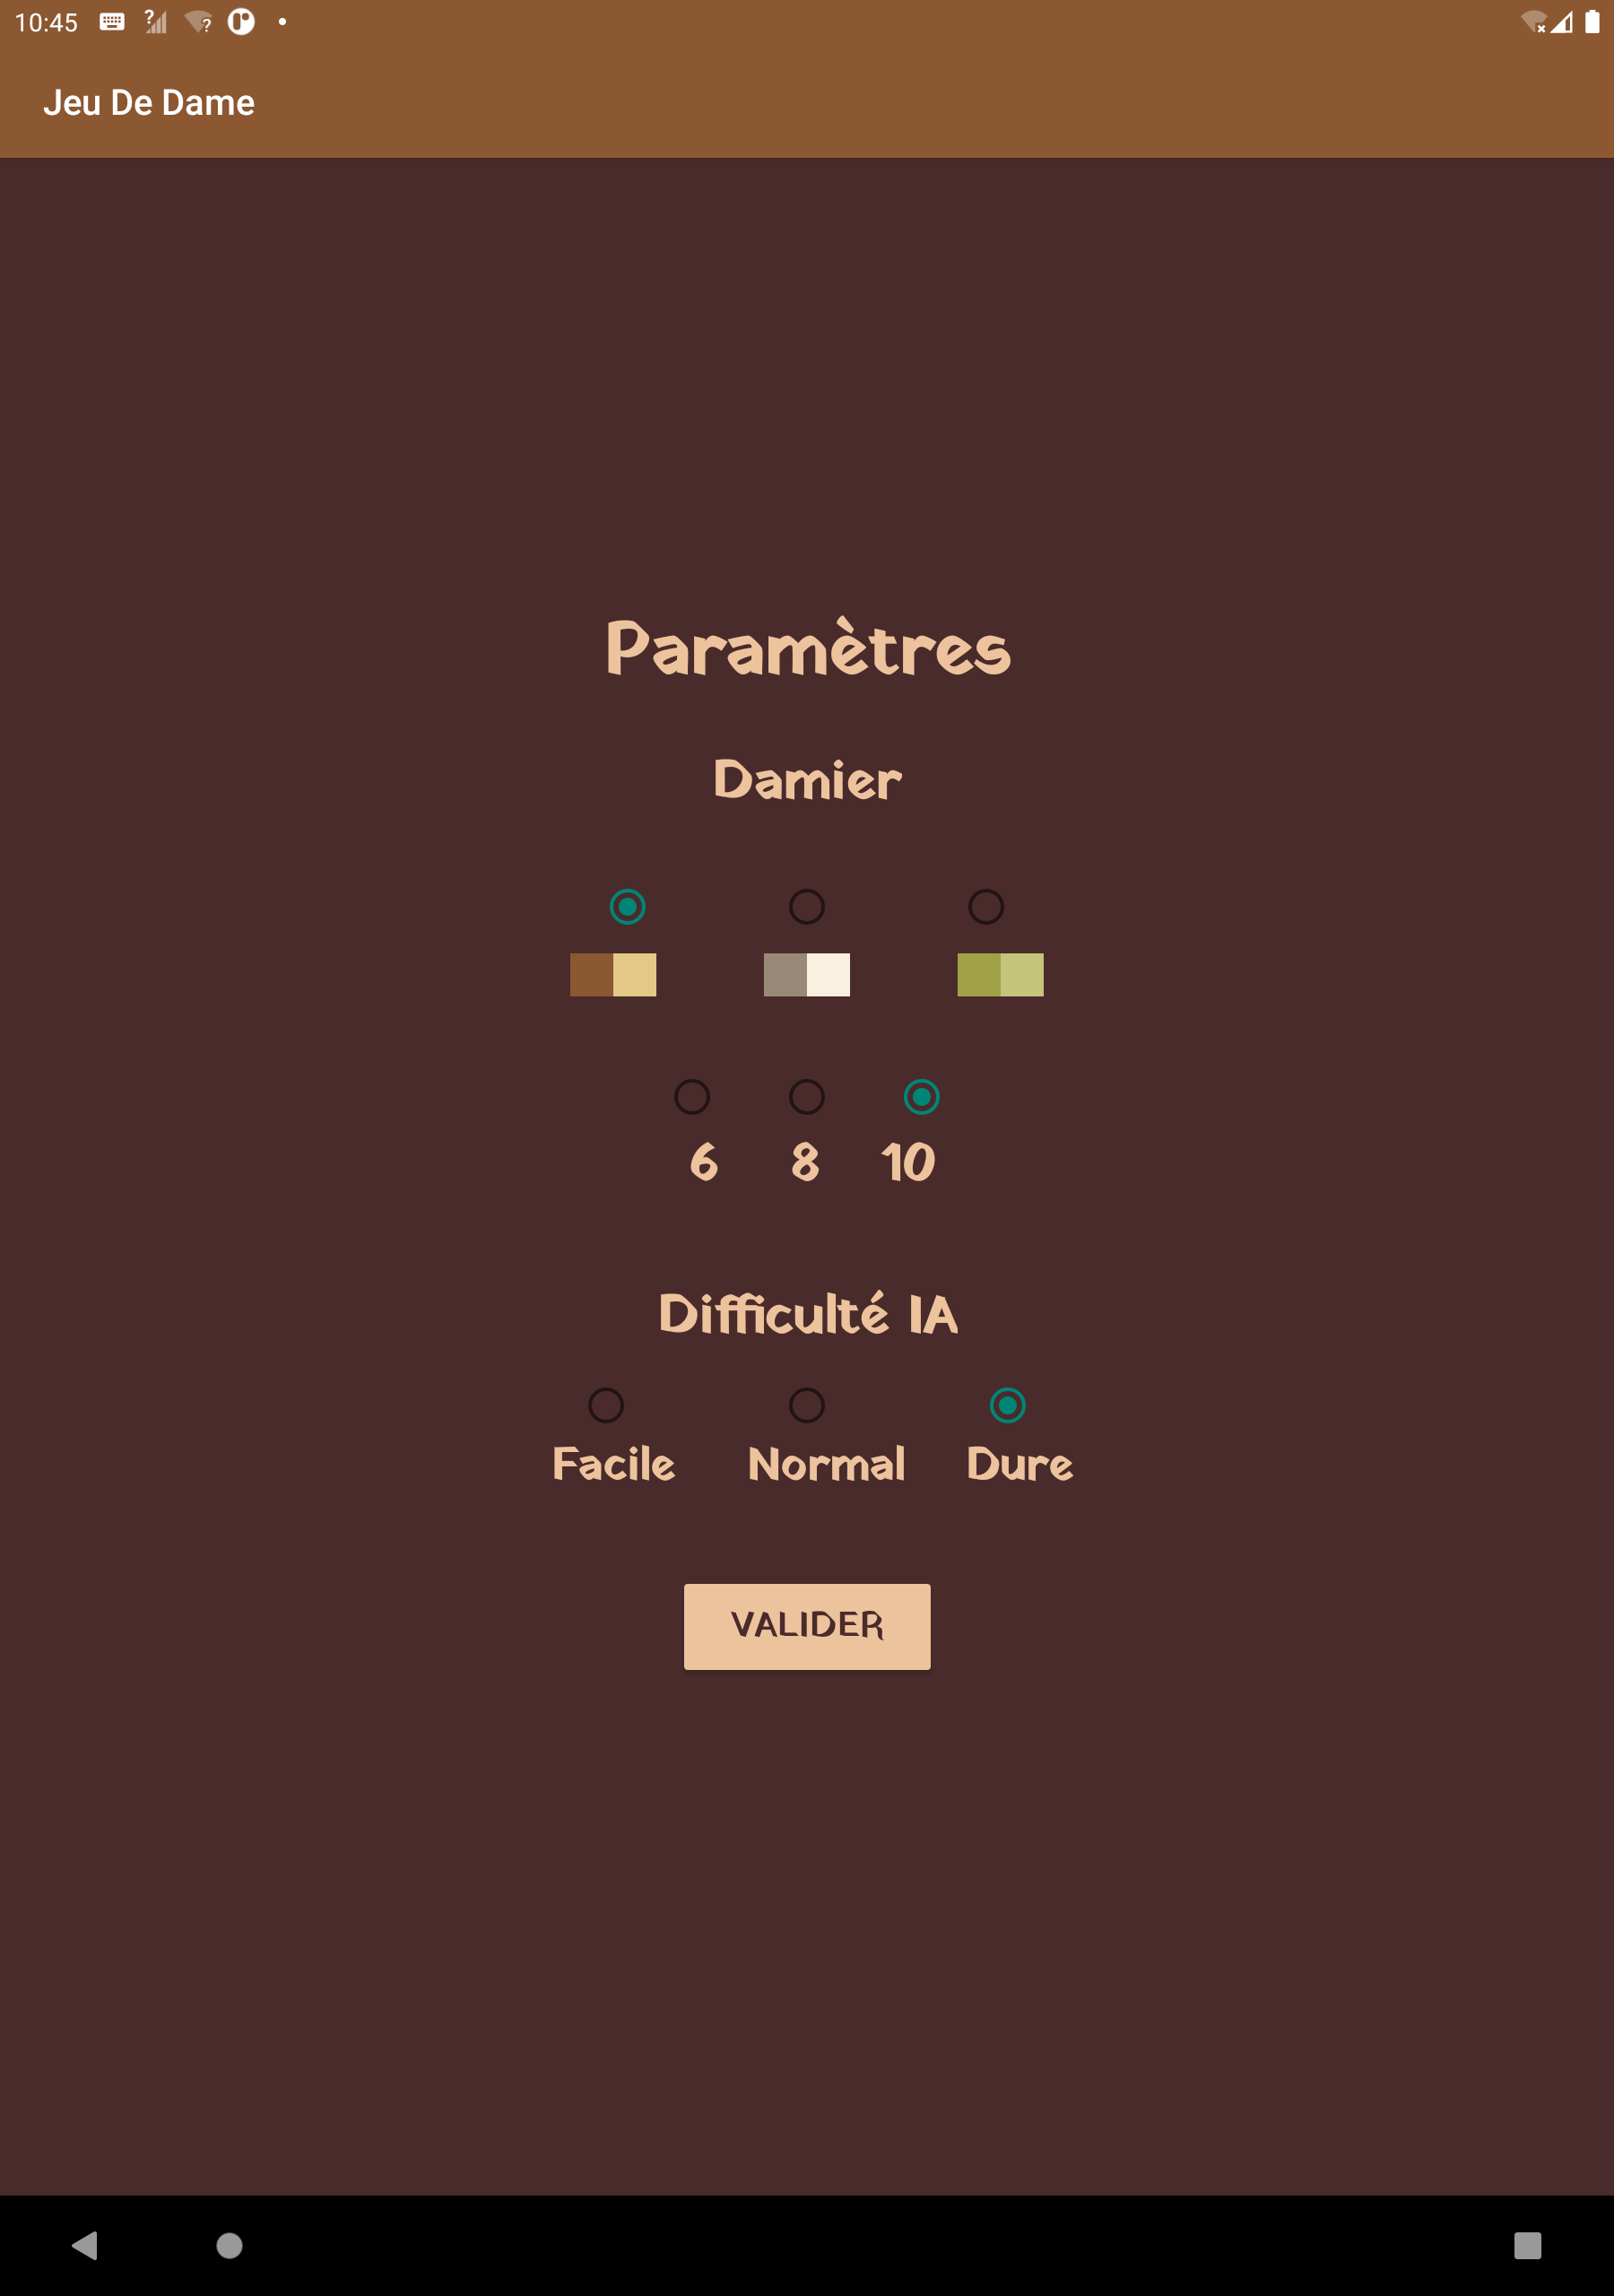
\includegraphics[scale=0.06]{setting_tablet_fr.png}
  \end{center}

  \begin{center}
    Totalement \textbf{responsive}
  
    Utilisation de \textbf{ConstraintLayout}
  \end{center}

\end{frame}

\begin{frame}
  \frametitle{Plateau de jeu}
  \subsection{Plateau de jeu}
  \begin{center}
    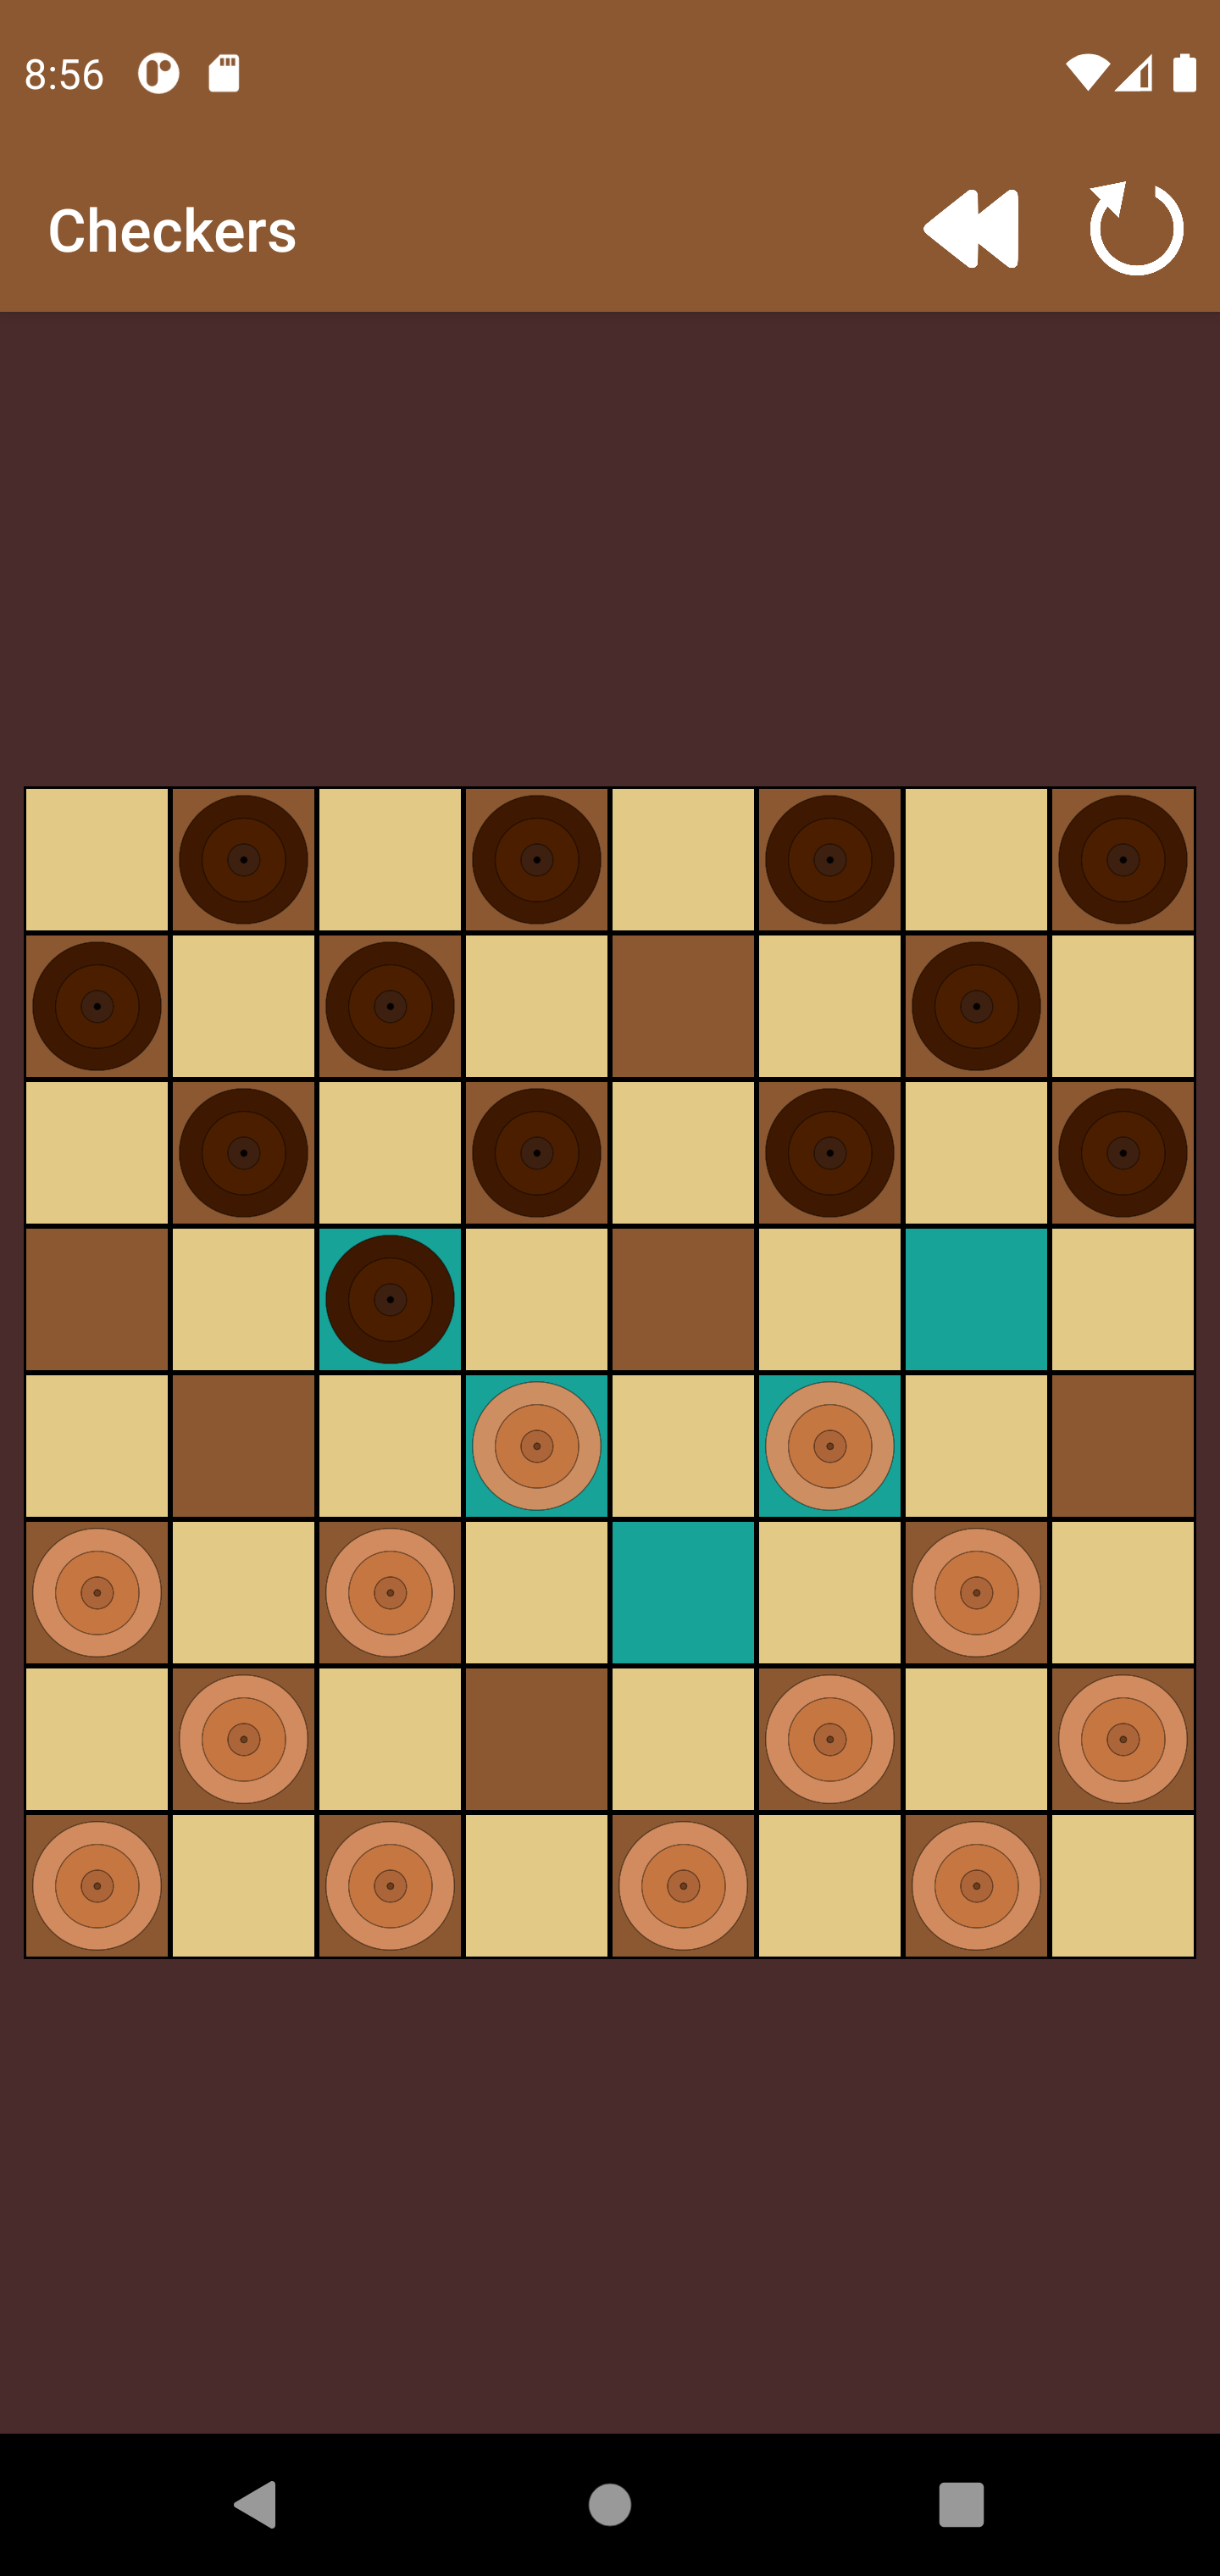
\includegraphics[scale=0.05]{partie_1.png}
    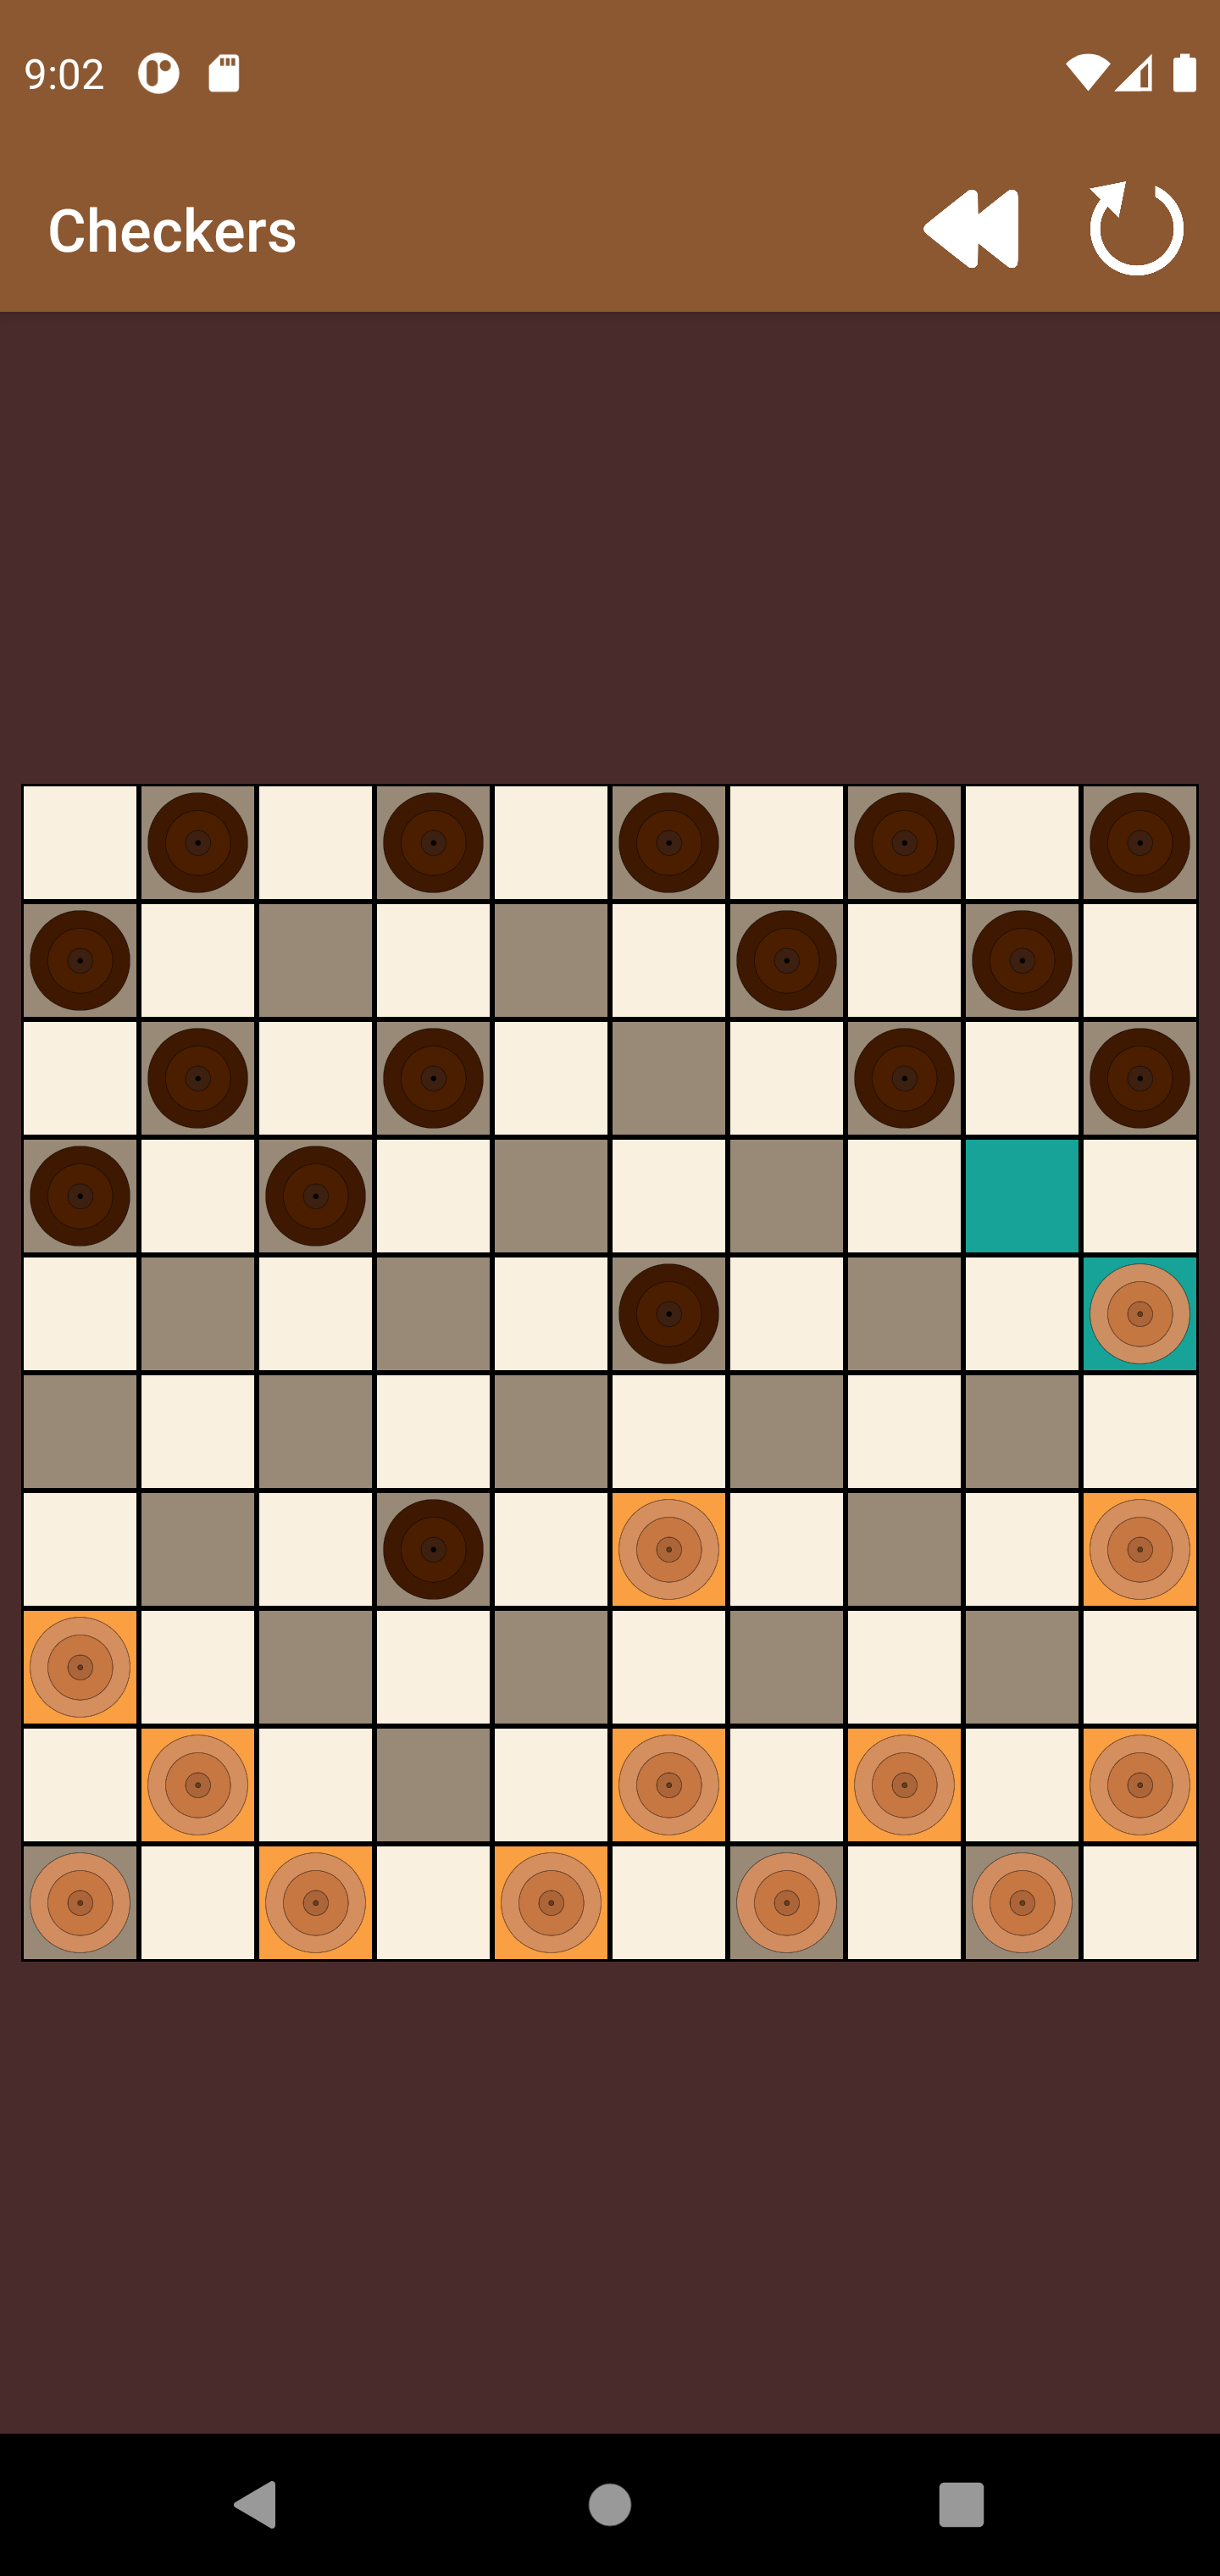
\includegraphics[scale=0.05]{partie_2.png}
    \begin{center}
      Bouton \textbf{Retour en arrière} et Bouton \textbf{Restart}
    \end{center}
  \end{center}

\end{frame}

\begin{frame}
  \frametitle{Plateau de jeu sur tablette}
  \begin{center}
    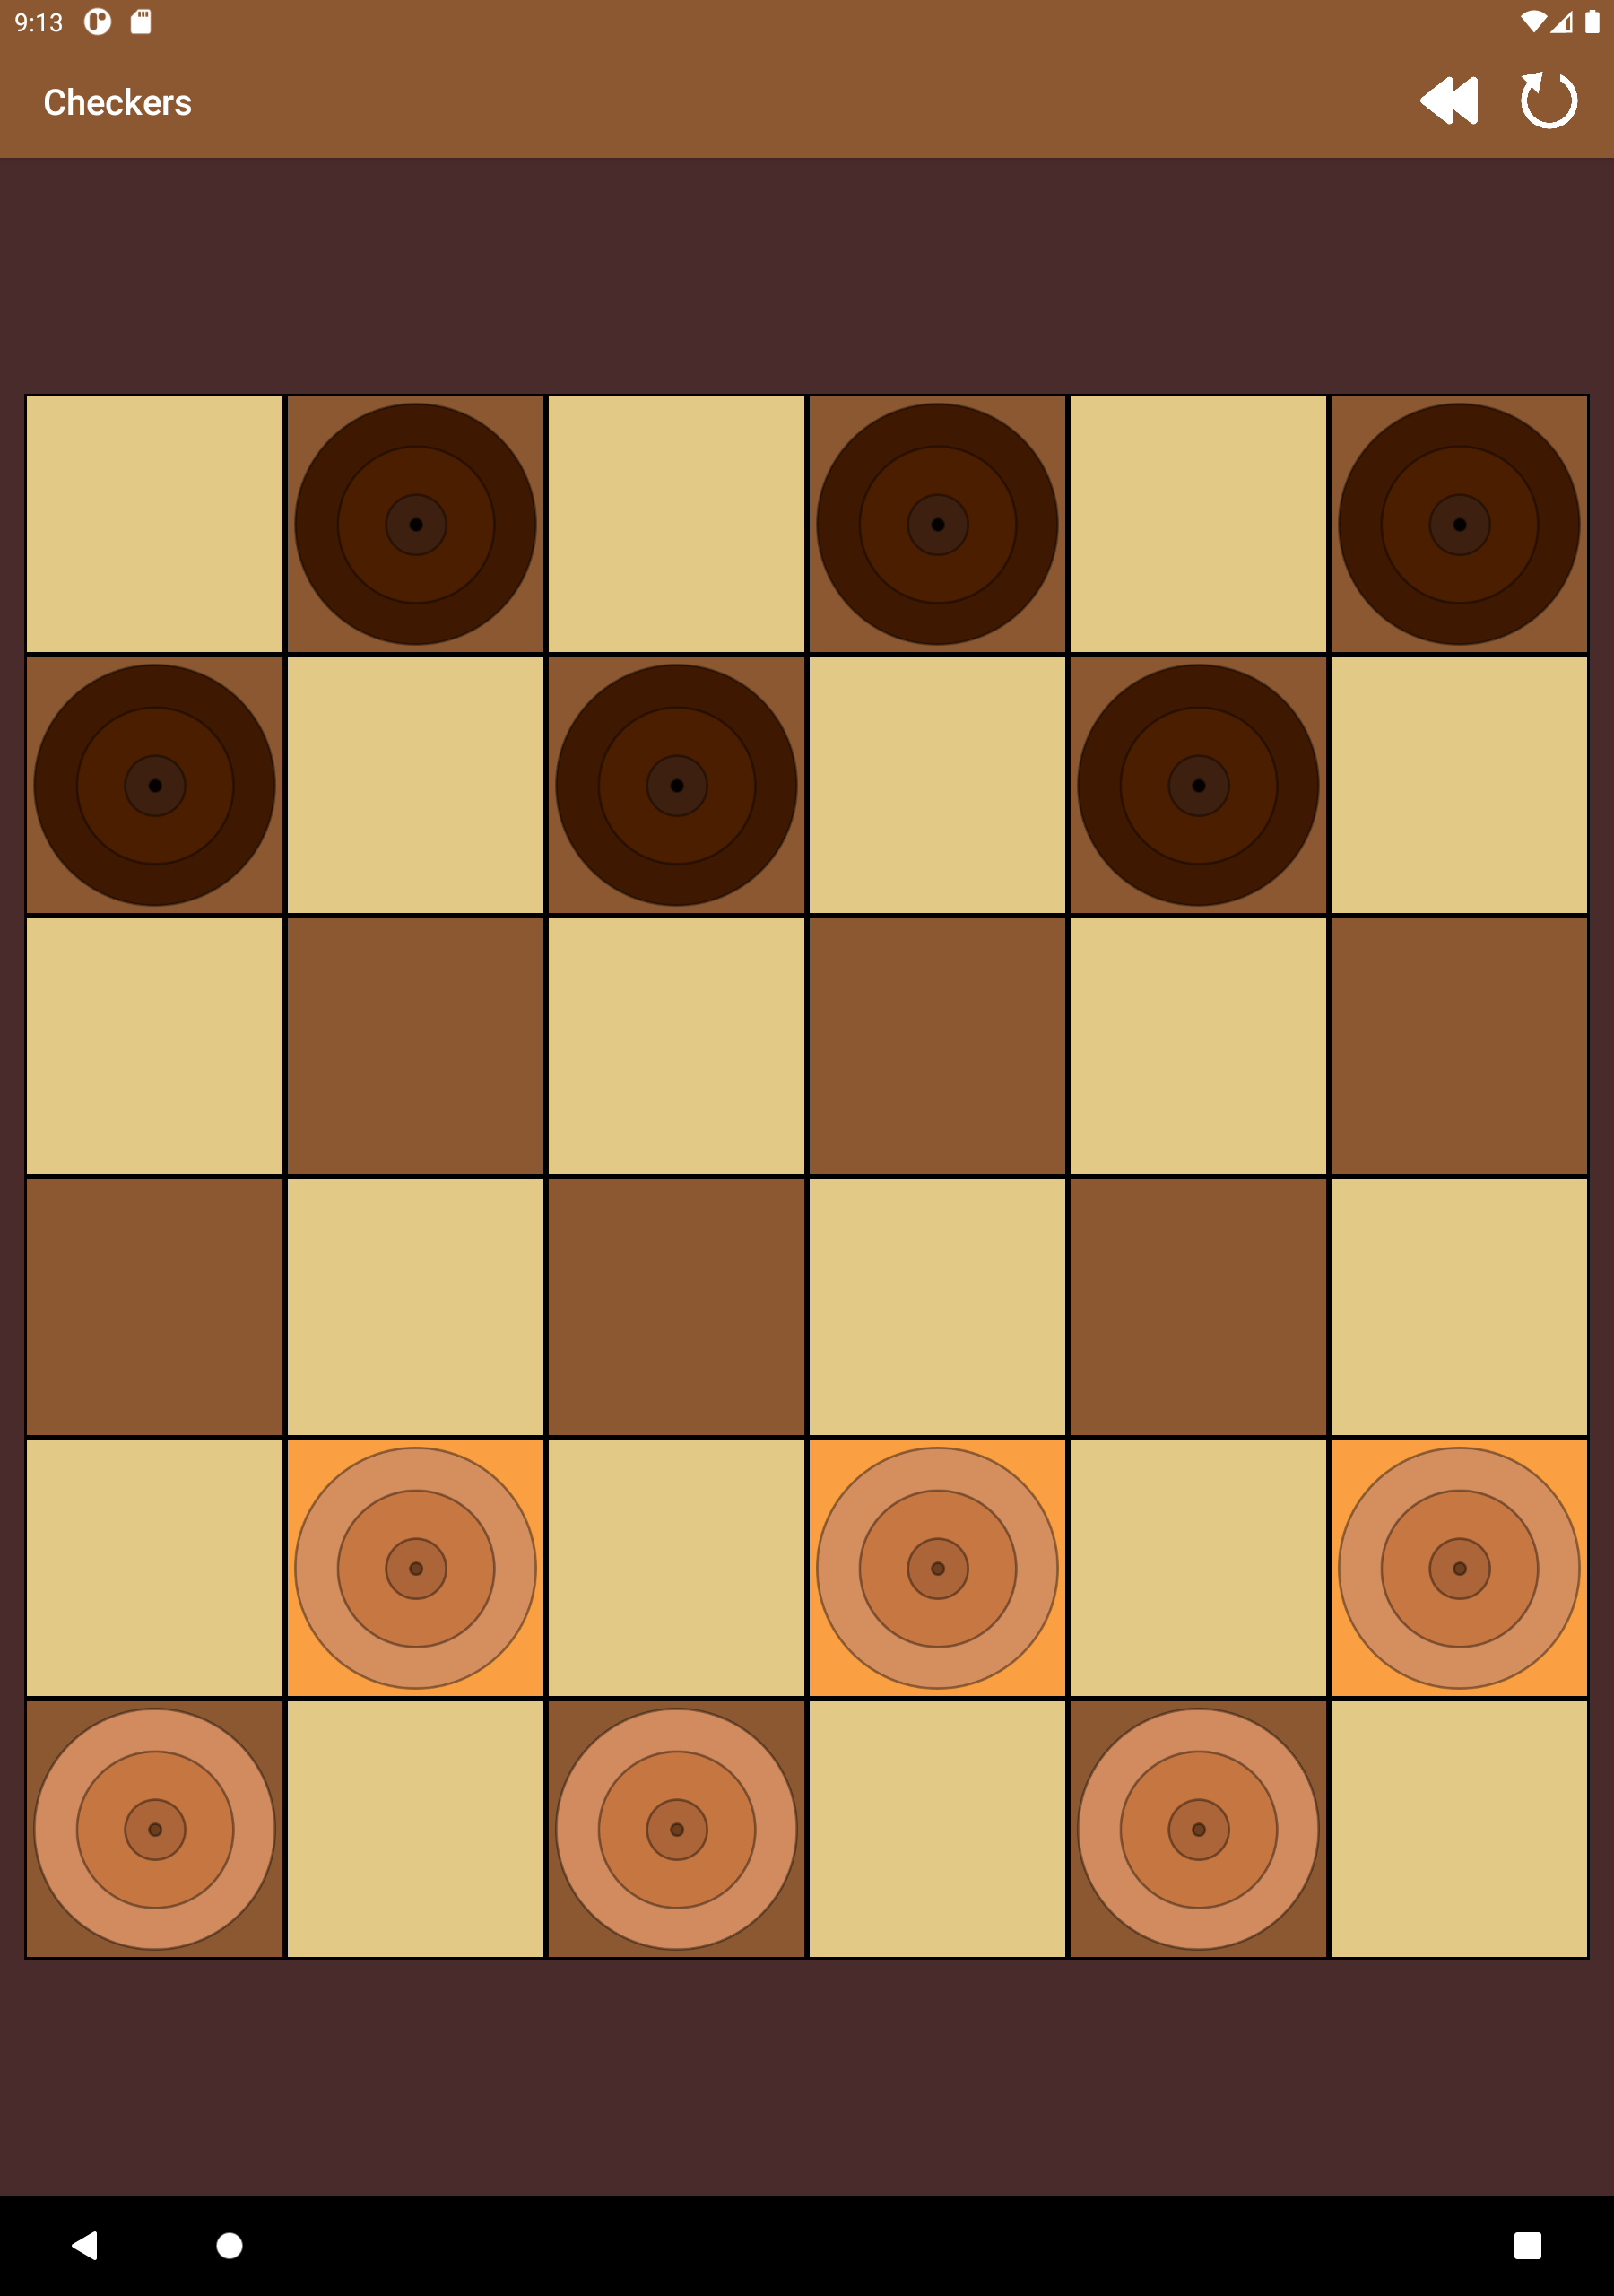
\includegraphics[scale=0.06]{screen_tablet.png}
  \end{center}
  
  \begin{center}
    Totalement \textbf{responsive}
  \end{center}
\end{frame}

\begin{frame}
  \frametitle{Plateau de jeu sur tablette}
  \begin{center}
    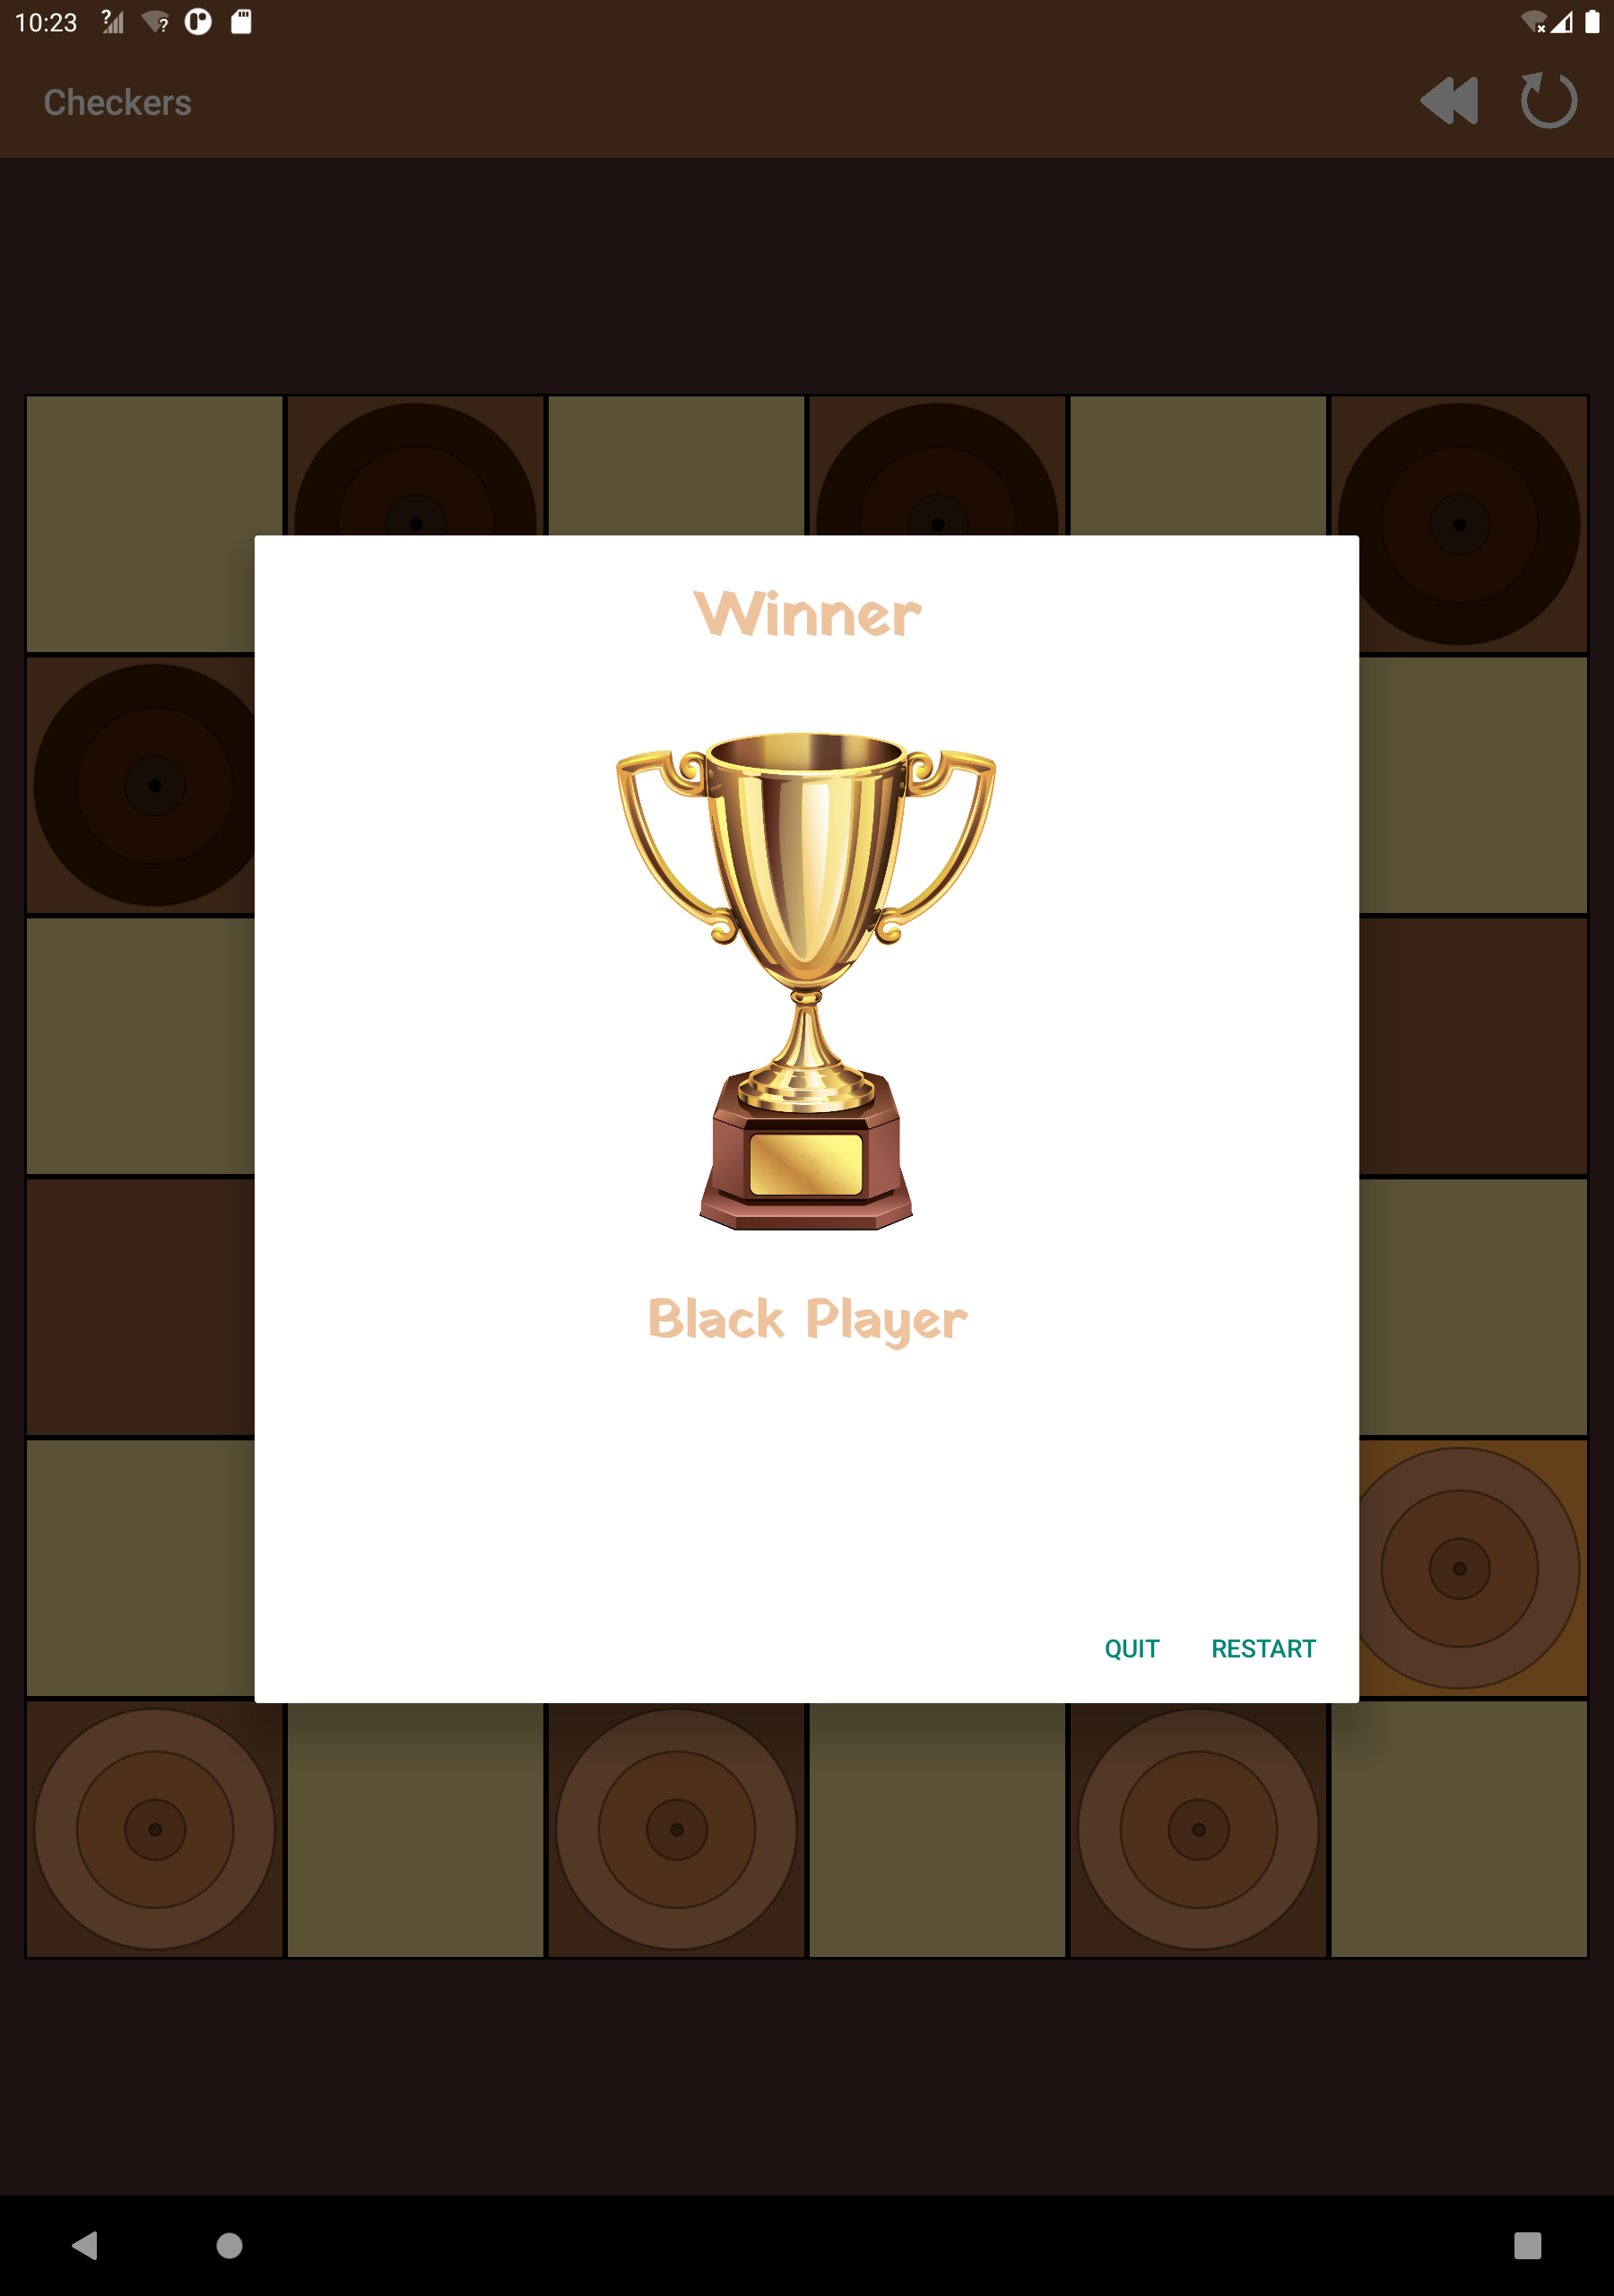
\includegraphics[scale=0.06]{pop_up_victoire_tablet.png}
  \end{center}
  
  \begin{center}
    Le pop up lorsqu'un joueur gagne la partie
  \end{center}
\end{frame}


%
%
%%%%%%%%%%%%%%%%%%%%%%%%%%%%%%%%%%%%
\section{Analyse du code}
%%%%%%%%%%%%%%%%%%%%%%%%%%%%%%%%%%%%
%
%
\begin{frame}
  \frametitle{Le model MVC}

  L'implémentation du jeu utilise le motifs d'architecture MVC

  \begin{itemize}
    \item \textbf{Model}: Permet de gerer toute la logique du Jeu
    \item \textbf{Vue}: Permet de gerer l'affichage
    \item \textbf{Controlleur}: Permet de faire le lien entre le model et la vue
  \end{itemize}

\end{frame}

\subsection{Diagramme UML}
\begin{frame}
  \frametitle{Diagramme UML}
  \begin{center}
    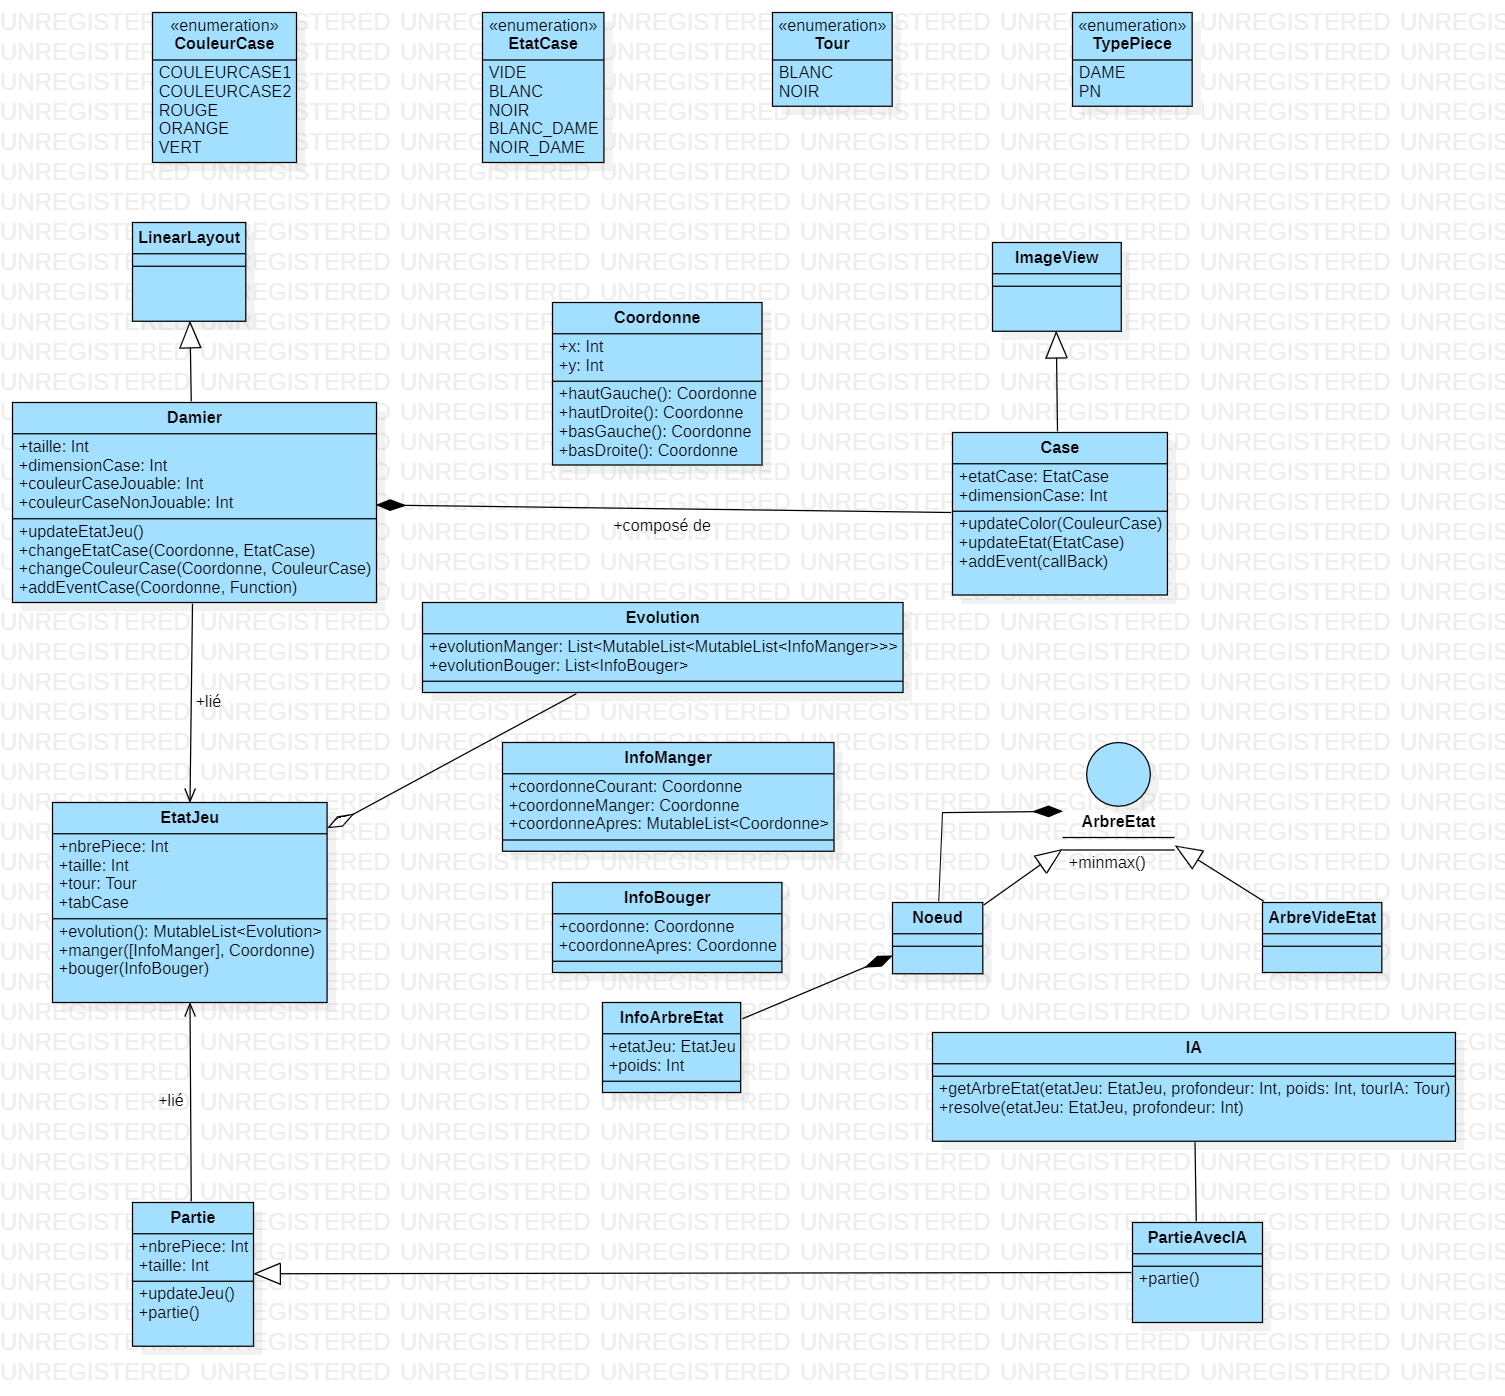
\includegraphics[scale=0.15]{diagramme_android.png}
  \end{center}
\end{frame}
%
%

\subsection{IA}

\begin{frame}
  \frametitle{Algorithme MiniMax}

  \begin{center}
    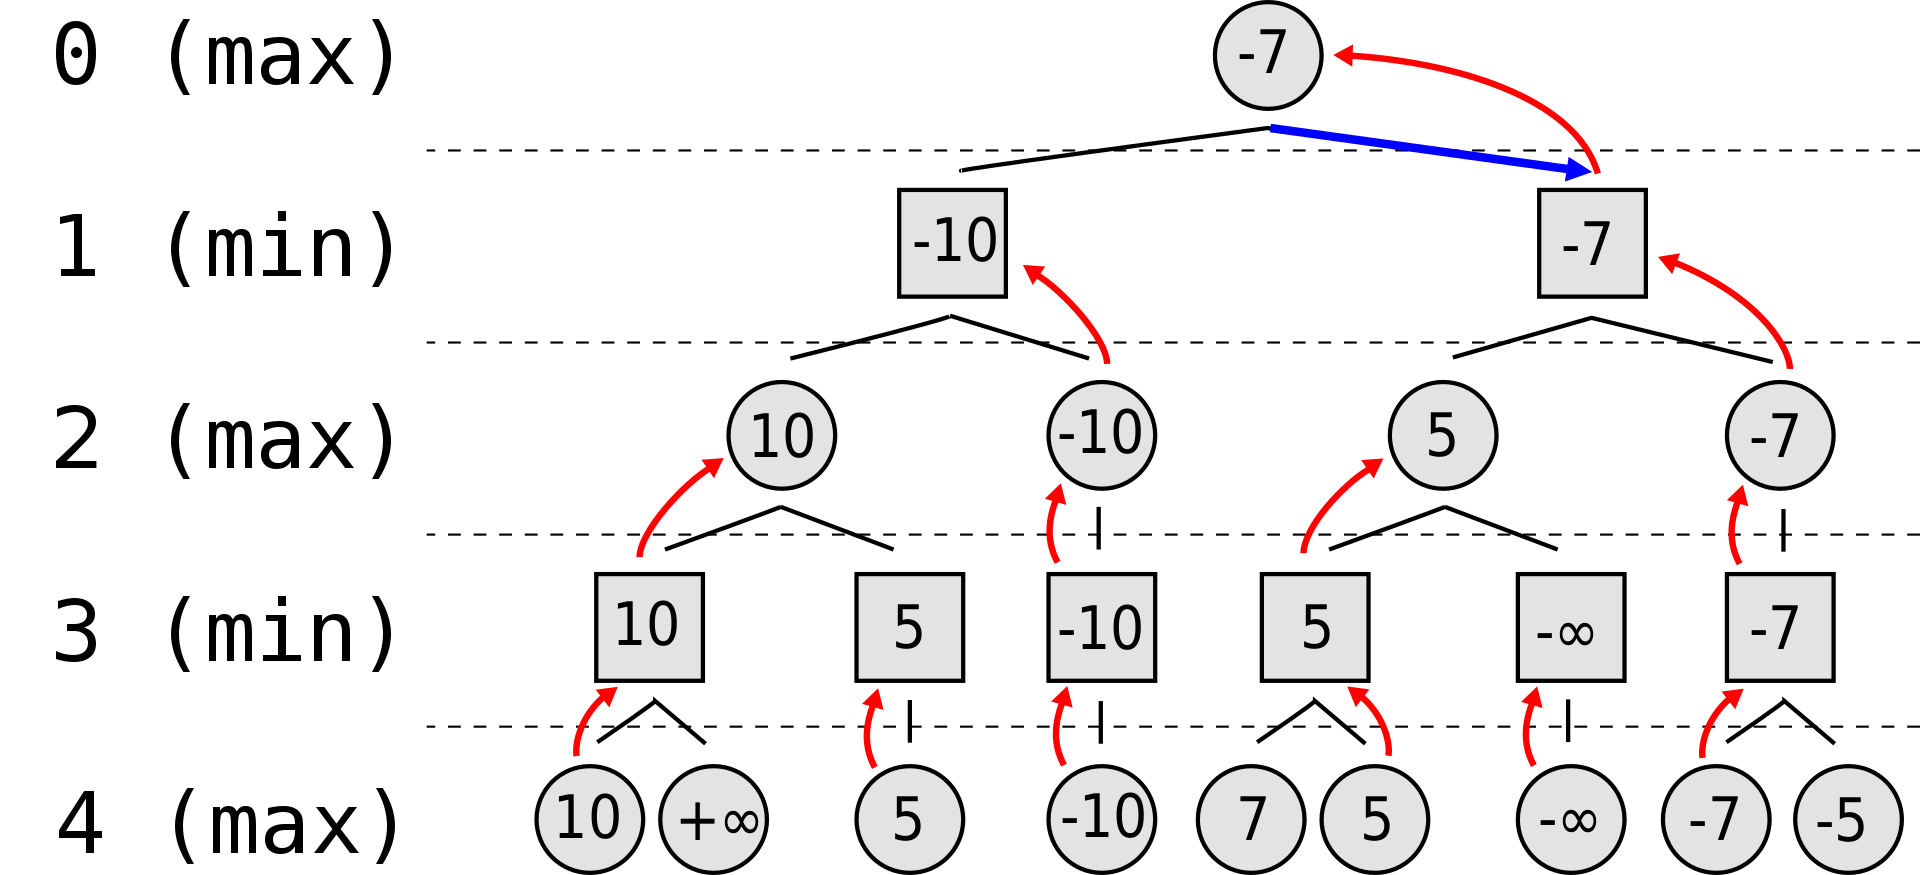
\includegraphics[scale=0.12]{minimax.png}
  \end{center}

  

\end{frame}

\begin{frame}
  \frametitle{IA}

  \begin{itemize}
    \item Le mode \textbf{joueur vs IA} met en jeu un IA 
    \item L'IA est implémenter avec l'algorithme minimax sans élagage alpha béta
    \item La fonction d'évalation corréspond au nombre de pions adverse pris, 
    soustrait au nombre de pions que l'adversaire nous a pris
    \item En effectuant l'algorithme sur une profondeur de 2,
    On a déja un IA capable de battre un débutant.
    \item L'Ia propose même des strategies très intérressants avec une profondeur de 4
    \item Pour des raisons de performances, 
    on pourra pas aller au dessus d'une profondeur de 6
  \end{itemize}

\end{frame}
%
%
%%%%%%%%%%%%%%%%%%%%%%%%%%%%%%%%%%%%
\section{Conclusion}
%%%%%%%%%%%%%%%%%%%%%%%%%%%%%%%%%%%%

\begin{frame}
  \frametitle{Point délicat}
  \subsection{Point délicat}
  \begin{itemize}
    \item Le paradigme orienté objet ?
    \item Compléxité du jeu de dame ?
    \item Syndrome de l'imposteur
  \end{itemize}

\end{frame}

\begin{frame}
  \frametitle{Point intéréssant}
  \subsection{Point intéréssant}
  \begin{itemize}
    \item Kotlin, le meilleur language de programmation ?
    \item L'IA, pas si durs que ça !
    \item Utilisation de tout les notions vue durant la licence !
  \end{itemize}

\end{frame}


\end{document}
